\documentclass[12pt, a4paper]{article}

% ==========================================
% 1. KHAI BÁO GÓI THƯ VIỆN (PACKAGES)
% ==========================================
% Bảng mã & Font chữ
\usepackage[utf8]{inputenc}
\usepackage[T5]{fontenc}

% Toán học
\usepackage{amsmath, amssymb}

% Căn lề & Bố cục trang
\usepackage[top=2.2cm, bottom=1.5cm, left=1cm, right=1cm, headheight=15pt]{geometry}
\usepackage{fancyhdr}
\usepackage{needspace}
\usepackage{tkz-tab}

% Đồ họa & Màu sắc
\usepackage{xcolor}
\usepackage{graphicx} 
\usepackage{tikz}
\usetikzlibrary{calc, shapes.geometric, positioning}


% Bảng biểu & Danh sách
\usepackage{colortbl}
\usepackage{array}
\usepackage{makecell}
\usepackage{multirow}
\usepackage{tasks}

% Biểu tượng
\usepackage{fontawesome5}

% ==========================================
% 2. THIẾT LẬP MÀU SẮC CHỦ ĐẠO
% ==========================================
\definecolor{goldyellow}{RGB}{255, 179, 0}
\definecolor{amberorange}{RGB}{230, 115, 0}
\definecolor{lightamber}{RGB}{255, 248, 225}
\definecolor{deepblue}{RGB}{25, 42, 86}
\definecolor{accentred}{RGB}{232, 65, 24}
\definecolor{softgray}{RGB}{220, 220, 222} 
\definecolor{fbblue}{RGB}{15, 80, 200}


% ==========================================
% 3. CẤU HÌNH HEADER & FOOTER
% ==========================================
\pagestyle{fancy}
\fancyhf{}
\renewcommand{\headrulewidth}{0pt}

% Khai báo biến lưu trữ nội dung góc phải của Header
\newcommand{\HeaderRightText}{}

% --- Header ---
\fancyhead[C]{
    \begin{tikzpicture}[remember picture, overlay]
        
        % Dải màu trang trí góc trên
        \path[fill=deepblue] (current page.north west) -- (current page.north east) 
            -- ($(current page.north east) + (0, -1.6cm)$) 
            .. controls ($(current page.north) + (3, -2.0cm)$) and ($(current page.north) + (-3, -0.4cm)$) .. 
            ($(current page.north west) + (0, -1.0cm)$) -- cycle;
            
        \path[fill=goldyellow] (current page.north west) -- (current page.north east) 
            -- ($(current page.north east) + (0, -1.0cm)$) 
            .. controls ($(current page.north) + (4, -1.0cm)$) and ($(current page.north) + (-2, -2.2cm)$) .. 
            ($(current page.north west) + (0, -1.6cm)$) -- cycle;
            
        \path[fill=amberorange] (current page.north west) -- ($(current page.north west) + (6.5cm, 0)$) 
            .. controls ($(current page.north west) + (4.5cm, -1.2cm)$) and ($(current page.north west) + (2cm, -2.0cm)$) .. 
            ($(current page.north west) + (0, -2.0cm)$) -- cycle;
            
        % Logo góc trái Header
        \node[anchor=west, inner sep=0pt] 
            at ($(current page.north west) + (0cm, -0.8cm)$) {
\includegraphics[height=2.0cm]{../../../image/logo-header.png}};
            
        % Text góc phải Header (Tự động lấy từ đối số thứ 3 của \titlebox)
        \node[anchor=east, text=white, font=\small\bfseries\sffamily] 
            at ($(current page.north east) + (-0.8cm, -0.5cm)$) {\HeaderRightText};
    \end{tikzpicture}
}

% --- Footer ---
\fancyfoot[C]{
    \begin{tikzpicture}[remember picture, overlay]
        % Đường kẻ ngang
        \draw[amberorange, line width=1.5pt] 
            ($(current page.south west) + (0cm, 0.4cm)$) -- ($(current page.south east) + (0cm, 0.4cm)$);

        % Dải cong góc phải
        \path[fill=goldyellow] (current page.south east) -- ($(current page.south east) + (-5cm, 0)$) 
            .. controls ($(current page.south east) + (-3cm, 0.8cm)$) and ($(current page.south east) + (-1.5cm, 1.2cm)$) .. 
            ($(current page.south east) + (0, 1.2cm)$) -- cycle;

        % Mạng xã hội
        \node[anchor=west, inner sep=0pt] at ($(current page.south west) + (1cm, 0.8cm)$) {
            \small\sffamily
            \textcolor{fbblue}{\faFacebook\hskip 4pt Toán Anh Huy MATH-STER}
            \hskip 18pt
            \textcolor{black}{\faTiktok\hskip 4pt huymathster}
        };

        % Số trang
        \node[circle, fill=white, draw=amberorange, line width=1.5pt, text=deepblue, font=\large\bfseries\sffamily, inner sep=4pt, minimum size=0.8cm] 
            at ($(current page.south east) + (-1.2cm, 0.6cm)$) {\thepage};
    \end{tikzpicture}
}

% ==========================================
% 4. ĐỊNH NGHĨA MACRO: KHUNG TIÊU ĐỀ
% ==========================================
\newcommand{\titlebox}[3]{
    % Gán nội dung đối số #3 vào biến HeaderRightText
    \gdef\HeaderRightText{#3}
    
    \begin{center}
    \vspace*{-0.5cm}
    \begin{tikzpicture}
        % Khung vô hình (Phantom Box) định chuẩn kích thước
        \node[text width=16cm, inner xsep=0pt, inner ysep=16pt, opacity=0] (MainBox) {
            \begin{minipage}[c]{4.2cm}
                \centering\vspace{0.1cm}
                \rule{2.2cm}{2.2cm} 
                \vspace{0.1cm}
            \end{minipage}%
            \begin{minipage}[c]{11.5cm}
                \centering\vspace{0.15cm}
                {\huge\bfseries\sffamily #2 \par}
                \vspace{0.15cm} 
            \end{minipage}
        };
        
        % Đổ bóng & Nền
        \fill[goldyellow, rounded corners=8pt] ([xshift=5pt, yshift=-5pt]MainBox.south west) rectangle ([xshift=5pt, yshift=-5pt]MainBox.north east);
        \fill[white, rounded corners=8pt] (MainBox.south west) rectangle (MainBox.north east);
        
        % Lưới ô ly & Nền Logo
        \begin{scope}
            \clip[rounded corners=8pt] (MainBox.south west) rectangle (MainBox.north east);
            \draw[step=0.4cm, softgray!50, line width=0.6pt] (MainBox.south west) grid (MainBox.north east);
            \fill[lightamber!60] (MainBox.south west) rectangle ([xshift=4.2cm]MainBox.north west);
        \end{scope}

        % Viền ngoài
        \draw[deepblue, line width=1.5pt, rounded corners=8pt] (MainBox.south west) rectangle (MainBox.north east);

        % Nội dung Text (Lớp trên cùng)
        \node[text width=16cm, inner xsep=0pt, inner ysep=16pt] at (MainBox.center) {
            \begin{minipage}[c]{4.2cm}
                \centering
                % --- ĐIỀU CHỈNH TỌA ĐỘ LOGO Ở ĐÂY ---
                \hspace*{-0.5cm}\raisebox{-0.2cm}{
\includegraphics[width=5.5cm]{../../../image/logo.png}}
            \end{minipage}%
            \begin{minipage}[c]{11.5cm}
                \centering\vspace{0.15cm}
                {\huge\bfseries\sffamily\color{deepblue} #2 \par}
                \vspace{0.15cm} 
            \end{minipage}
        };
        
        % Trang trí phụ kiện
        \draw[deepblue, line width=1.5pt, dashed] ([xshift=4.2cm]MainBox.north west) -- ([xshift=4.2cm]MainBox.south west);
        \node[regular polygon, regular polygon sides=4, rotate=45, fill=white, draw=accentred, line width=1.2pt, inner sep=2.5pt] at ([xshift=4.2cm]MainBox.west) {};
        \node[anchor=west, fill=amberorange, text=white, font=\large\bfseries\sffamily, rounded corners=4pt, draw=deepblue, line width=1.5pt, inner xsep=12pt, inner ysep=6pt] at ([xshift=1.5cm]MainBox.north west) {#1};
        \fill[accentred] ([xshift=-1.8cm, yshift=-0.4cm]MainBox.north east) circle (3pt);
        \fill[amberorange] ([xshift=-1.4cm, yshift=-0.4cm]MainBox.north east) circle (3pt);
        \fill[goldyellow] ([xshift=-1.0cm, yshift=-0.4cm]MainBox.north east) circle (3pt);
    \end{tikzpicture}
    \vspace*{0cm}
    \end{center}
}

% ==========================================
% 5. ĐỊNH NGHĨA MACRO: CẤU TRÚC CÂU HỎI (ÉP SÁT NHAU)
% ==========================================
\newcommand{\questioncore}[2]{
    % Xóa khoảng cách phía trên, ép sát câu trước
    \noindent \textbf{\textcolor{deepblue}{Câu #1.} \textcolor{accentred}{[STER]}} #2
    \par\nopagebreak
}

% Cấu hình hiển thị đáp án trắc nghiệm
\settasks{
    label=\textbf{\textcolor{amberorange}{\Alph*.}}, 
    label-width=15pt,     
    item-indent=25pt,     
    label-offset=6pt,    
    column-sep=20pt,     
    after-item-skip=2pt  % Đã giảm tối đa khoảng cách giữa các dòng đáp án A B C D
}

% Hàm vẽ dòng kẻ nháp
\newcommand{\drawdashlines}[1]{
    \ifnum#1>0
        \nopagebreak\vspace{0.1cm}\noindent 
        \begin{tikzpicture}
            \foreach \i in {1,...,#1} {
                \draw[softgray, line width=0.2pt] (0,-{\i*0.65}) -- (\textwidth-4pt,-{\i*0.65});
            }
        \end{tikzpicture}
        \par
    \fi
    % Đã xóa hoàn toàn khoảng cách thừa ở nhánh else
}

% --- Dạng 1: Trắc nghiệm 4 đáp án ---
\newcommand{\questionLinesManual}[4]{
    \pgfmathsetmacro{\calculatedSpace}{1.5 + #1 * 0.65}
    \needspace{\calculatedSpace cm} 
    \questioncore{#2}{#3}
    #4
    \par\nopagebreak
    \drawdashlines{#1}
}

% --- Dạng 2: Trắc nghiệm Đúng/Sai ---
\newcommand{\questionTrueFalse}[4]{
    \pgfmathsetmacro{\calculatedSpace}{3.0 + #1 * 0.65} 
    \needspace{\calculatedSpace cm}
    \questioncore{#2}{#3}
    
    \nopagebreak
    \begin{center}
    \renewcommand{\arraystretch}{1.2} % Bóp nhỏ chiều cao của bảng Đ/S
    \begin{tabular}{|>{\centering\arraybackslash}m{0.8cm}|m{12cm}|>{\centering\arraybackslash}m{2cm}|>{\centering\arraybackslash}m{2cm}|}
        \hline
        \rowcolor{amberorange!20}
        & \multicolumn{1}{>{\centering\arraybackslash}m{12cm}|}{\textbf{\textcolor{deepblue}{Mệnh đề}}} & 
        \textbf{\textcolor{deepblue}{Đúng}} & 
        \textbf{\textcolor{deepblue}{Sai}} \\
        \hline
        #4
        \hline
    \end{tabular}
    \renewcommand{\arraystretch}{1}
    \end{center}
    
    \par\nopagebreak
    \drawdashlines{#1}
}

% ----- Dạng 3: Tự luận ngắn -----
\newcommand{\questionShortAnswer}[3]{
    \pgfmathsetmacro{\calculatedSpace}{1.5 + #1 * 0.8}
    \needspace{\calculatedSpace cm}
    
    {\linespread{1.1}\selectfont % Bóp nhỏ giãn dòng của câu tự luận
    \questioncore{#2}{#3}\par}
    
    \nopagebreak
    \begin{flushright}
        \begin{tikzpicture}
            \node[anchor=east, font=\small\bfseries\sffamily, text=deepblue] 
                at (-0.2, 0.4) {Đáp án:};
            \fill[goldyellow, rounded corners=3pt] (0.08, -0.08) rectangle (3.08, 0.72);
            \draw[draw=deepblue, fill=white, line width=1.2pt, rounded corners=3pt] 
                (0,0) rectangle (3.0, 0.8);
            \foreach \x in {0.75, 1.5, 2.25} {
                \draw[draw=deepblue, line width=0.6pt] (\x, 0) -- (\x, 0.8);
            }
        \end{tikzpicture}
    \end{flushright}
    
    \par\nopagebreak
    \drawdashlines{#1}
}

% ==========================================
% BẮT ĐẦU NỘI DUNG TÀI LIỆU
% ==========================================
\begin{document}

% Truyền 3 tham số: {Nhãn cam} {Chữ to chính giữa} {Chữ ở góc phải Header}
\titlebox{Chủ đề: Hàm số}{Đường tiện cận}{Hàm số: Đường tiện cận}

% --- CÂU 1 ---
\questionLinesManual{0}{1}{Cho hàm số \( y = \dfrac{ax + b}{cx + d} \), (\(ac \neq 0, ad - bc \neq 0\)) có bảng biến thiên như dưới đây.

\begin{center}
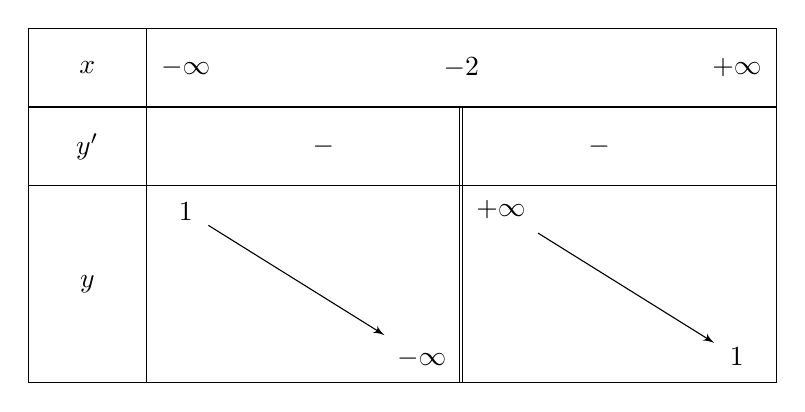
\begin{tikzpicture}
    \tkzTabInit[lgt=1.5, espcl=3.5]
    {$x$ /1, $y'$ /1, $y$ /2.5}
    {$-\infty$, $-2$, $+\infty$}
    \tkzTabLine{, -, d, -, }
    \tkzTabVar{+/ $1$ / , -D+/ $-\infty$ / $+\infty$ , -/ $1$ /}
\end{tikzpicture}
\end{center}

Đường tiệm cận đứng của đồ thị hàm số đã cho có phương trình là}{
    \begin{tasks}(4)
        \task \(y = -2\)
        \task \(x = 1\)
        \task \(y = 1\)
        \task \(x = -2\)
    \end{tasks}
}

% --- CÂU 2 ---
\questionLinesManual{0}{2}{Cho hàm số \( y = f(x) \) có bảng biến thiên như hình vẽ dưới đây.

\begin{center}
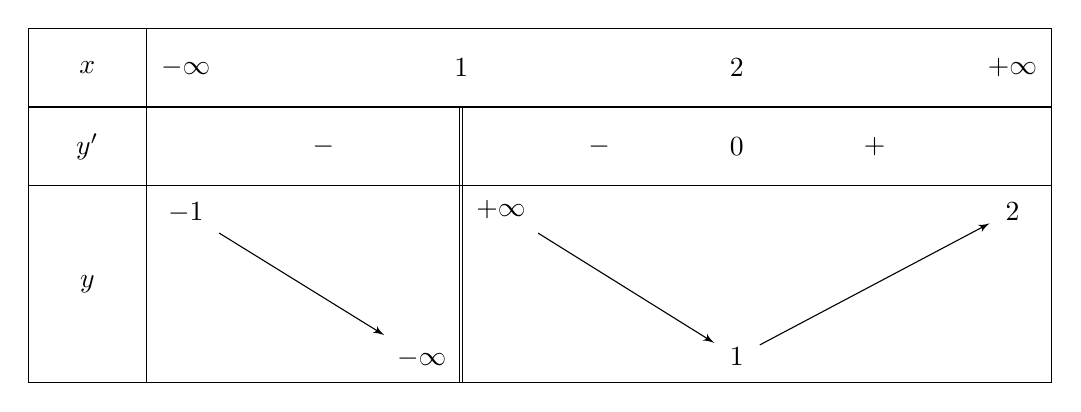
\begin{tikzpicture}
    \tkzTabInit[lgt=1.5, espcl=3.5]
    {$x$ /1, $y'$ /1, $y$ /2.5}
    {$-\infty$, $1$, $2$, $+\infty$}
    \tkzTabLine{, -, d, -, 0, +, }
    \tkzTabVar{+/ $-1$ / , -D+/ $-\infty$ / $+\infty$ , -/ $1$ / , +/ $2$ /}
\end{tikzpicture}
\end{center}

Đồ thị hàm số \( y = f(x) \) có bao nhiêu đường tiệm cận?}{
    \begin{tasks}(4)
        \task $3$
        \task $2$
        \task $1$
        \task $4$
    \end{tasks}
}

% --- CÂU 3 ---
\questionLinesManual{0}{3}{Cho hàm số \( f(x) \) xác định trên \( (-\infty; 0) \setminus \{-2\} \) và có bảng biến thiên bên dưới. Đồ thị hàm số đã cho có tổng số đường tiệm cận ngang và tiệm cận đứng là

\begin{center}
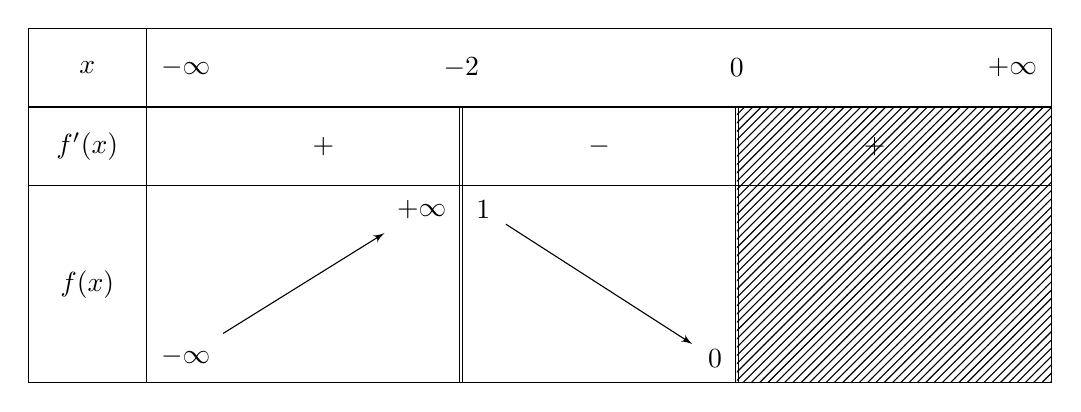
\begin{tikzpicture}
    \tkzTabInit[lgt=1.5, espcl=3.5]
    {$x$ /1, $f'(x)$ /1, $f(x)$ /2.5}
    {$-\infty$, $-2$, $0$, $+\infty$}
    \tkzTabLine{, +, d, -, d,+}
    \tkzTabVar{-/ $-\infty$ / , +D+/ $+\infty$ / $1$, -D/ $0$ /}
   \fill[pattern=north east lines](9,-4.5) rectangle (13,-1);
\end{tikzpicture}
\end{center}}{
    \begin{tasks}(4)
        \task $1$
        \task $3$
        \task $0$
        \task $2$
    \end{tasks}
}

% --- CÂU 4 ---
\questionLinesManual{0}{4}{Cho hàm số \( y = f(x) \) xác định trên \( \mathbb{R} \setminus \{1\} \), liên tục trên mỗi khoảng xác định và có bảng biến thiên như hình bên dưới. Hỏi đồ thị hàm số đã cho có tất cả bao nhiêu đường tiệm cận đứng và đường tiệm cận ngang?

\begin{center}
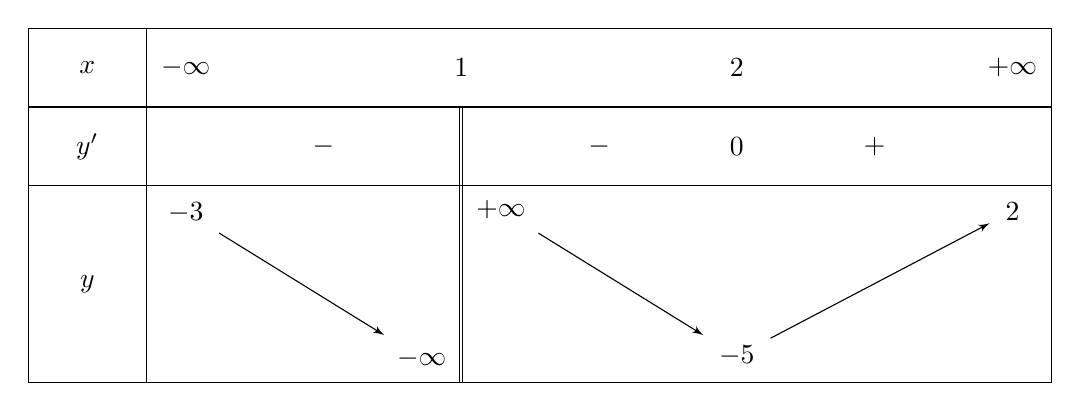
\begin{tikzpicture}
    \tkzTabInit[lgt=1.5, espcl=3.5]
    {$x$ /1, $y'$ /1, $y$ /2.5}
    {$-\infty$, $1$, $2$, $+\infty$}
    \tkzTabLine{, -, d, -, 0, +, }
    \tkzTabVar{+/ $-3$ / , -D+/ $-\infty$ / $+\infty$ , -/ $-5$ / , +/ $2$ /}
\end{tikzpicture}
\end{center}

}{
    \begin{tasks}(4)
        \task $1$
        \task $2$
        \task $3$
        \task $4$
    \end{tasks}
}

\questionLinesManual{0}{5}{Cho hàm số \( y = \dfrac{ax + b}{cx + d} \) (\(ad - bc \neq 0\); \(c \neq 0\)) có bảng biến thiên như sau

\begin{center}
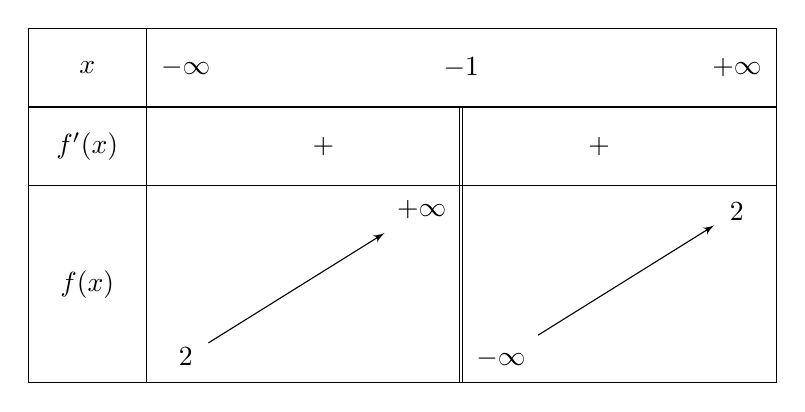
\begin{tikzpicture}
    \tkzTabInit[lgt=1.5, espcl=3.5]
    {$x$ /1, $f'(x)$ /1, $f(x)$ /2.5}
    {$-\infty$, $-1$, $+\infty$}
    \tkzTabLine{, +, d, +, }
    \tkzTabVar{-/ $2$ / , +D-/ $+\infty$ / $-\infty$, +/ $2$ /}
\end{tikzpicture}
\end{center}

Đồ thị hàm số có đường tiệm cận đứng là}{
    \begin{tasks}(4)
        \task \( y = -1 \)
        \task \( y = 2 \)
        \task \( x = 2 \)
        \task \( x = -1 \)
    \end{tasks}
}

% --- CÂU 6 ---
\questionLinesManual{0}{6}{Cho hàm số \( y = f(x) \) có bảng biến thiên như sau:

\begin{center}
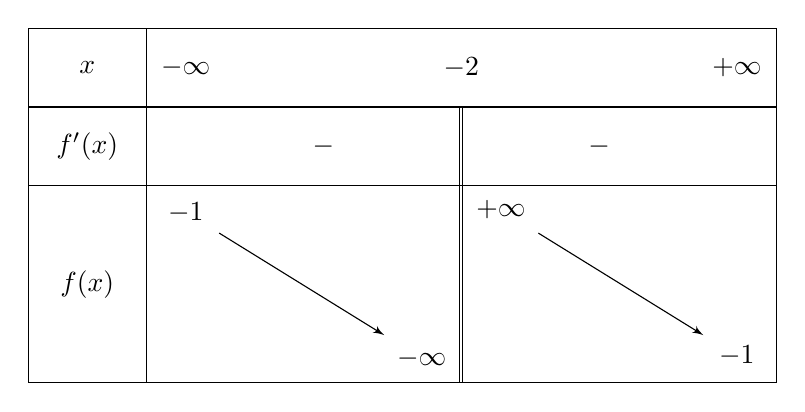
\begin{tikzpicture}
    \tkzTabInit[lgt=1.5, espcl=3.5]
    {$x$ /1, $f'(x)$ /1, $f(x)$ /2.5}
    {$-\infty$, $-2$, $+\infty$}
    \tkzTabLine{, -, d, -, }
    \tkzTabVar{+/ $-1$ / , -D+/ $-\infty$ / $+\infty$ , -/ $-1$ /}
\end{tikzpicture}
\end{center}

Tiệm cận đứng của đồ thị hàm số đã cho là đường thẳng có phương trình:}{
    \begin{tasks}(4)
        \task \( x = -1 \)
        \task \( x = -2 \)
        \task \( y = -1 \)
        \task \( y = -2 \)
    \end{tasks}
}

% --- CÂU 7 ---
\questionLinesManual{0}{7}{Cho hàm số \( y = f(x) \) xác định trên \( \mathbb{R} \setminus \{1\} \), liên tục trên mỗi khoảng xác định và có bảng biến thiên như sau:

\begin{center}
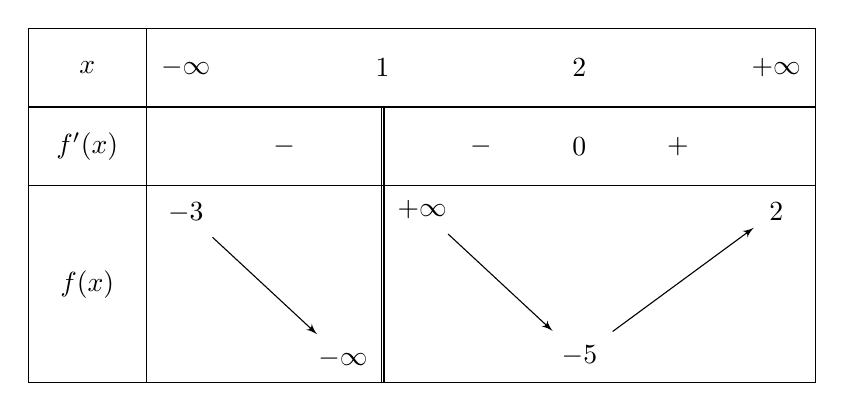
\begin{tikzpicture}
    \tkzTabInit[lgt=1.5, espcl=2.5]
    {$x$ /1, $f'(x)$ /1, $f(x)$ /2.5}
    {$-\infty$, $1$, $2$, $+\infty$}
    \tkzTabLine{, -, d, -, 0, +, }
    \tkzTabVar{+/ $-3$ / , -D+/ $-\infty$ / $+\infty$ , -/ $-5$ / , +/ $2$ /}
\end{tikzpicture}
\end{center}

Hỏi đồ thị hàm số đã cho có tất cả bao nhiêu đường tiệm cận đứng?}{
    \begin{tasks}(4)
        \task $4$
        \task $2$
        \task $3$
        \task $1$
    \end{tasks}
}

% --- CÂU 8 ---
\questionLinesManual{0}{8}{Cho hàm số \( y = f(x) \) có bảng biến thiên như sau:

\begin{center}
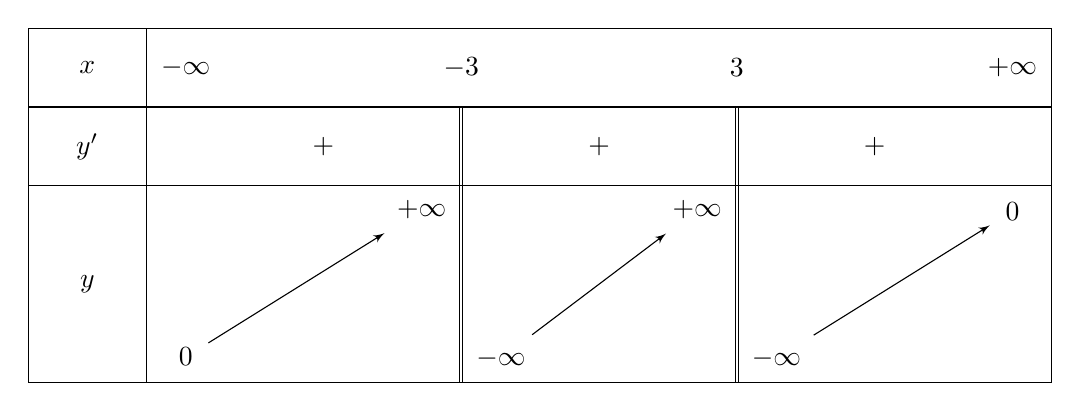
\begin{tikzpicture}
    \tkzTabInit[lgt=1.5, espcl=3.5]
    {$x$ /1, $y'$ /1, $y$ /2.5}
    {$-\infty$, $-3$, $3$, $+\infty$}
    \tkzTabLine{, +, d, +, d, +, }
    \tkzTabVar{-/ $0$ / , +D-/ $+\infty$ / $-\infty$, +D-/ $+\infty$ / $-\infty$, +/ $0$ /}
\end{tikzpicture}
\end{center}

Số đường tiệm cận đứng của đồ thị hàm số là}{
    \begin{tasks}(4)
        \task $4$
        \task $3$
        \task $2$
        \task $1$
    \end{tasks}
}

% --- CÂU 9 ---
\questionLinesManual{0}{9}{Cho hàm số \( y = f(x) \) xác định trên \( \mathbb{R} \setminus \{1\} \), liên tục trên mỗi khoảng xác định và có bảng biến thiên như hình bên dưới. Hỏi đồ thị hàm số đã cho có tất cả bao nhiêu đường tiệm cận đứng và đường tiệm cận ngang?

\begin{center}
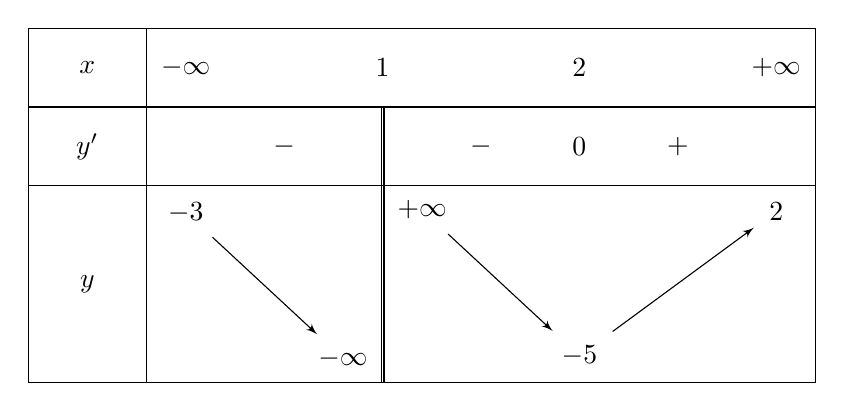
\begin{tikzpicture}
    \tkzTabInit[lgt=1.5, espcl=2.5]
    {$x$ /1, $y'$ /1, $y$ /2.5}
    {$-\infty$, $1$, $2$, $+\infty$}
    \tkzTabLine{, -, d, -, 0, +, }
    \tkzTabVar{+/ $-3$ / , -D+/ $-\infty$ / $+\infty$ , -/ $-5$ / , +/ $2$ /}
\end{tikzpicture}
\end{center}

}{
    \begin{tasks}(4)
        \task $1$
        \task $2$
        \task $3$
        \task $4$
    \end{tasks}
}

% --- CÂU 10 ---
\questionLinesManual{0}{10}{Cho hàm số \( y = f(x) \) có bảng biến thiên như sau

\begin{center}
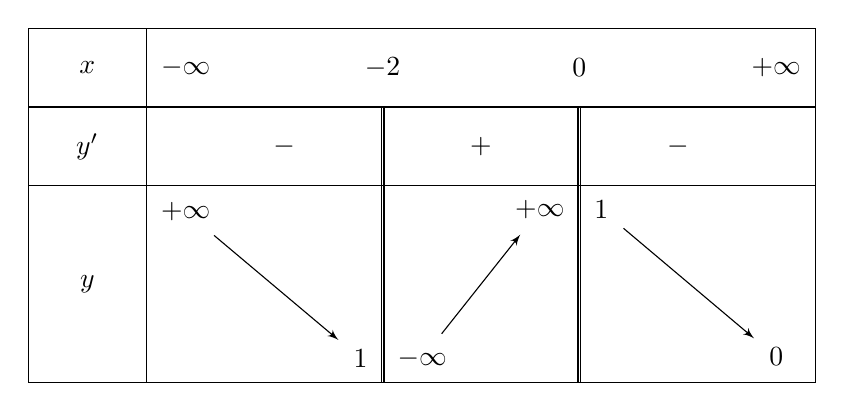
\begin{tikzpicture}
    \tkzTabInit[lgt=1.5, espcl=2.5]
    {$x$ /1, $y'$ /1, $y$ /2.5}
    {$-\infty$, $-2$, $0$, $+\infty$}
    \tkzTabLine{, -, d, +, d, -, }
    \tkzTabVar{+/ $+\infty$ / , -D-/ $1$ / $-\infty$/ ,+D+/ $+\infty$ / $1$ , -/ $0$ /}
\end{tikzpicture}
\end{center}

Tổng số đường tiệm cận đứng và tiệm cận ngang của đồ thị hàm số đã cho bằng}{
    \begin{tasks}(4)
        \task $3$
        \task $2$
        \task $1$
        \task $0$
    \end{tasks}
}

% --- CÂU 11 ---
\questionLinesManual{0}{11}{Cho hàm số \( y = f(x) \) có bảng biến thiên như sau:

\begin{center}
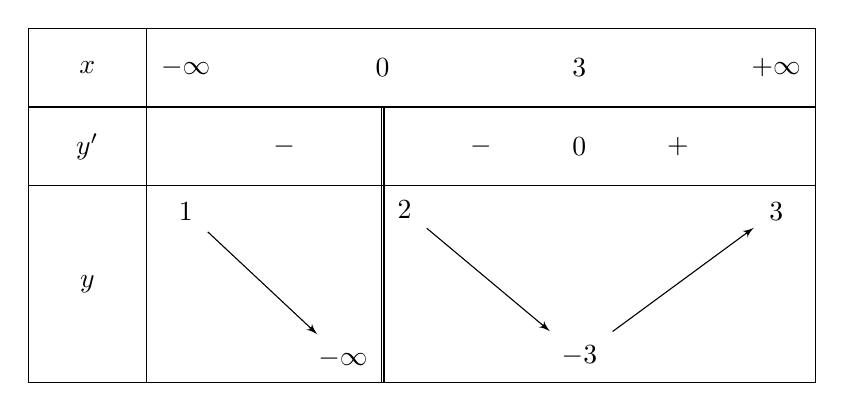
\begin{tikzpicture}
    \tkzTabInit[lgt=1.5, espcl=2.5]
    {$x$ /1, $y'$ /1, $y$ /2.5}
    {$-\infty$, $0$, $3$, $+\infty$}
    \tkzTabLine{, -, d, -, 0, +, }
    \tkzTabVar{+/ $1$ / , -D+/ $-\infty$ / $2$ , -/ $-3$ / , +/ $3$ /}
\end{tikzpicture}
\end{center}

Tổng số tiệm cận đứng và tiệm cận ngang của đồ thị hàm số đã cho là}{
    \begin{tasks}(4)
        \task $4$
        \task $2$
        \task $1$
        \task $3$
    \end{tasks}
}

% --- CÂU 12 ---
\questionLinesManual{0}{12}{Cho hàm số \( y = f(x) \) có bảng biến thiên như sau:

\begin{center}
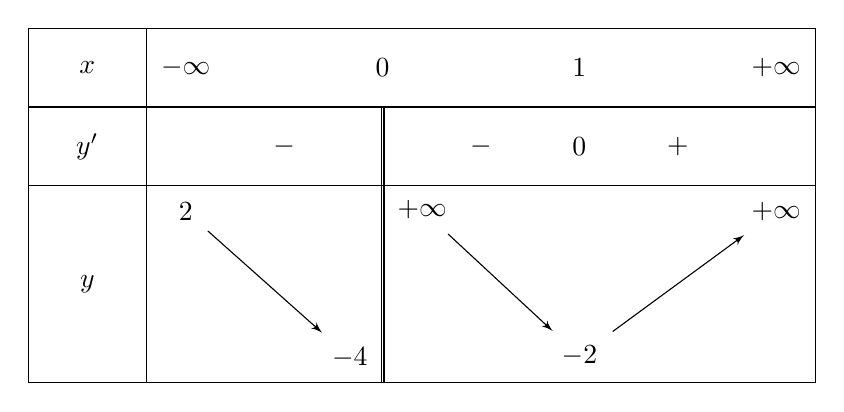
\begin{tikzpicture}
    \tkzTabInit[lgt=1.5, espcl=2.5]
    {$x$ /1, $y'$ /1, $y$ /2.5}
    {$-\infty$, $0$, $1$, $+\infty$}
    \tkzTabLine{, -, d, -, 0, +, }
    \tkzTabVar{+/ $2$ / , -D+/ $-4$ / $+\infty$ , -/ $-2$ / , +/ $+\infty$ /}
\end{tikzpicture}
\end{center}

Tổng số đường tiệm cận đứng và tiệm cận ngang của đồ thị hàm số đã cho là}{
    \begin{tasks}(4)
        \task $2$
        \task $4$
        \task $1$
        \task $3$
    \end{tasks}
}

% --- CÂU 13 ---
\questionLinesManual{0}{13}{Cho hàm số \( y = f(x) \) xác định trên \( \mathbb{R} \setminus \{-1\} \) có bảng biến thiên như hình bên

\begin{center}
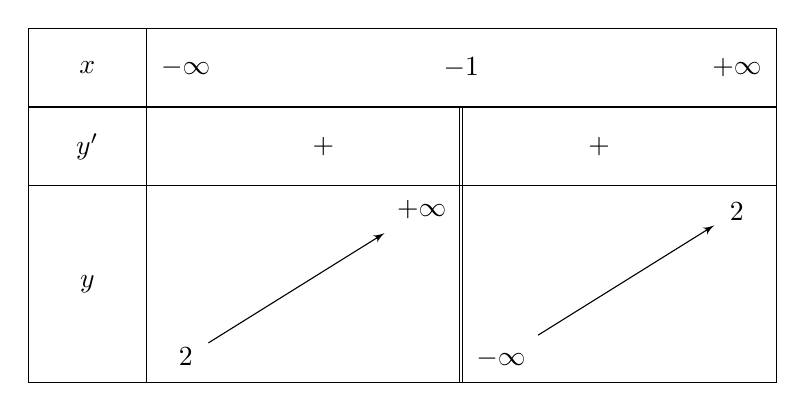
\begin{tikzpicture}
    \tkzTabInit[lgt=1.5, espcl=3.5]
    {$x$ /1, $y'$ /1, $y$ /2.5}
    {$-\infty$, $-1$, $+\infty$}
    \tkzTabLine{, +, d, +, }
    \tkzTabVar{-/ $2$ / , +D-/ $+\infty$ / $-\infty$, +/ $2$ /}
\end{tikzpicture}
\end{center}

Đồ thị hàm số \( y = f(x) \) có bao nhiêu đường tiệm cận ngang?}{
    \begin{tasks}(4)
        \task $0$
        \task $2$
        \task $3$
        \task $1$
    \end{tasks}
}

% --- CÂU 14 ---
\questionLinesManual{0}{14}{Cho hàm số \( y = f(x) \) liên tục trên \( \mathbb{R} \) và có bảng biến thiên như sau

\begin{center}
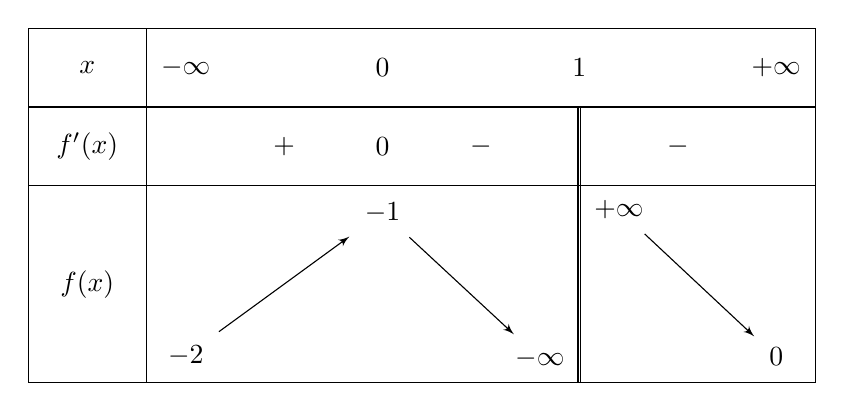
\begin{tikzpicture}
    \tkzTabInit[lgt=1.5, espcl=2.5]
    {$x$ /1, $f'(x)$ /1, $f(x)$ /2.5}
    {$-\infty$, $0$, $1$, $+\infty$}
    \tkzTabLine{, +, 0, -, d, -, }
    \tkzTabVar{-/ $-2$ / , +/ $-1$ / , -D+/ $-\infty$ / $+\infty$ , -/ $0$ /}
\end{tikzpicture}
\end{center}

Đồ thị hàm số \( y = \dfrac{1}{2f(x) + 3} \) có bao nhiêu đường tiệm cận đứng?}{
    \begin{tasks}(4)
        \task $3$
        \task $4$
        \task $2$
        \task $6$
    \end{tasks}
}

% --- CÂU 15 ---
\questionLinesManual{0}{15}{Cho hàm số \( y = f(x) \) có bảng biến thiên như sau:

\begin{center}
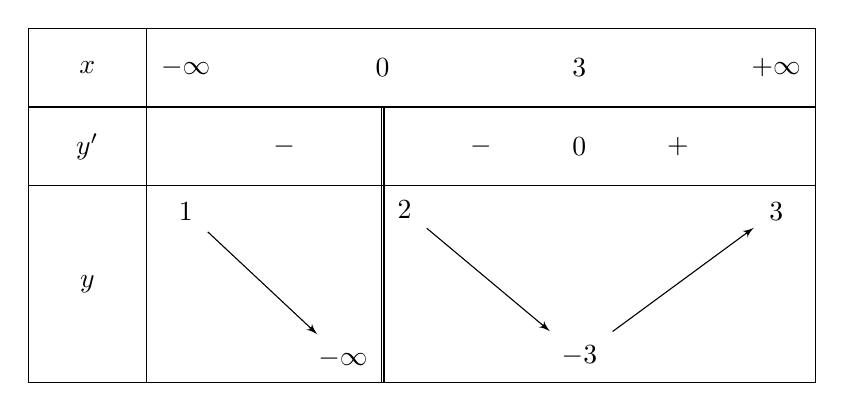
\begin{tikzpicture}
    \tkzTabInit[lgt=1.5, espcl=2.5]
    {$x$ /1, $y'$ /1, $y$ /2.5}
    {$-\infty$, $0$, $3$, $+\infty$}
    \tkzTabLine{, -, d, -, 0, +, }
    \tkzTabVar{+/ $1$ / , -D+/ $-\infty$ / $2$ , -/ $-3$ / , +/ $3$ /}
\end{tikzpicture}
\end{center}

Tổng số tiệm cận đứng và tiệm cận ngang của đồ thị hàm số đã cho là:}{
    \begin{tasks}(4)
        \task $2$
        \task $3$
        \task $4$
        \task $1$
    \end{tasks}
}

% --- CÂU 16 ---
\questionLinesManual{0}{16}{Cho hàm số \( f(x) \) có bảng biến thiên như sau

\begin{center}
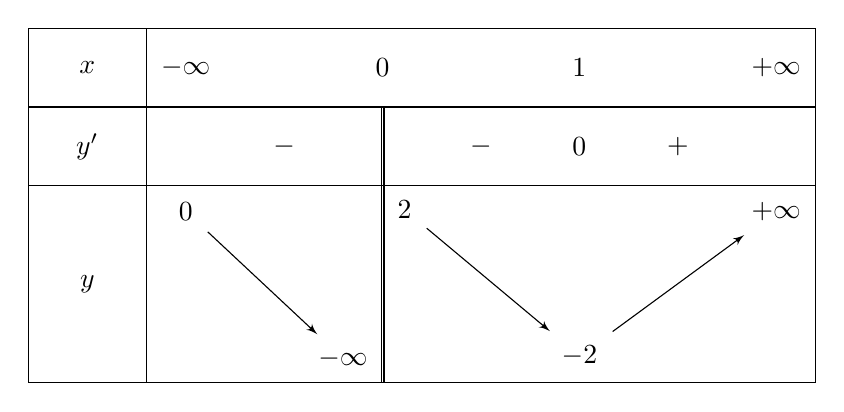
\begin{tikzpicture}
    \tkzTabInit[lgt=1.5, espcl=2.5]
    {$x$ /1, $y'$ /1, $y$ /2.5}
    {$-\infty$, $0$, $1$, $+\infty$}
    \tkzTabLine{, -, d, -, 0, +, }
    \tkzTabVar{+/ $0$ / , -D+/ $-\infty$ / $2$ , -/ $-2$ / , +/ $+\infty$ /}
\end{tikzpicture}
\end{center}

Tổng số tiệm cận đứng và tiệm cận ngang của đồ thị hàm số đã cho là}{
    \begin{tasks}(4)
        \task $1$
        \task $2$
        \task $4$
        \task $3$
    \end{tasks}
}

% --- CÂU 17 ---
\questionLinesManual{0}{17}{Cho hàm số \( y = f(x) \) có bảng biến thiên như sau:

\begin{center}
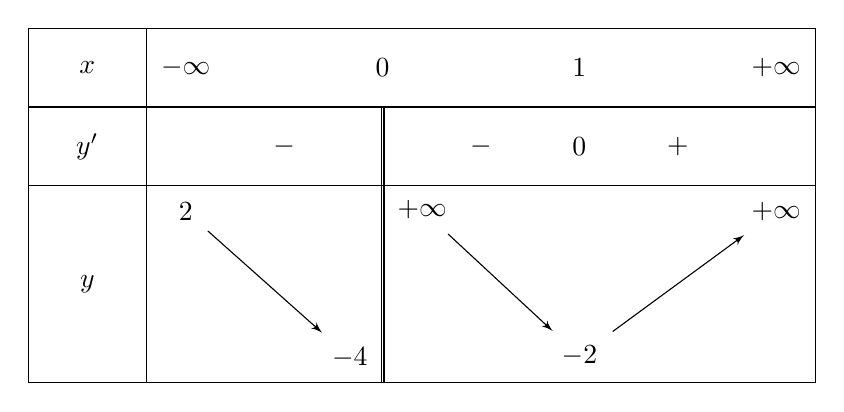
\begin{tikzpicture}
    \tkzTabInit[lgt=1.5, espcl=2.5]
    {$x$ /1, $y'$ /1, $y$ /2.5}
    {$-\infty$, $0$, $1$, $+\infty$}
    \tkzTabLine{, -, d, -, 0, +, }
    \tkzTabVar{+/ $2$ / , -D+/ $-4$ / $+\infty$ , -/ $-2$ / , +/ $+\infty$ /}
\end{tikzpicture}
\end{center}

Tổng số tiệm cận đứng và tiệm cận ngang của đồ thị hàm số đã cho là:}{
    \begin{tasks}(4)
        \task $4$
        \task $1$
        \task $3$
        \task $2$
    \end{tasks}
}

% --- CÂU 18 ---
\questionLinesManual{0}{18}{Cho hàm số \( y = f(x) \) có bảng biến thiên như sau

\begin{center}
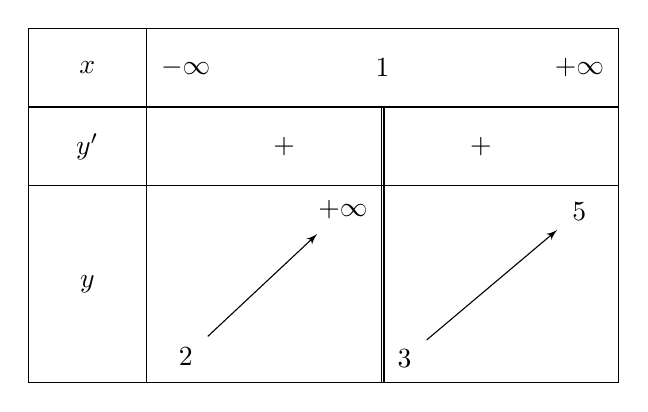
\begin{tikzpicture}
    \tkzTabInit[lgt=1.5, espcl=2.5]
    {$x$ /1, $y'$ /1, $y$ /2.5}
    {$-\infty$, $1$, $+\infty$}
    \tkzTabLine{, +, d, +, }
    \tkzTabVar{-/ $2$ / , +D-/ $+\infty$ / $3$ , +/ $5$ /}
\end{tikzpicture}
\end{center}

Tổng số đường tiệm cận ngang và đường tiệm cận đứng của đồ thị hàm số đã cho là}{
    \begin{tasks}(4)
        \task $3$
        \task $2$
        \task $4$
        \task $1$
    \end{tasks}
}

% --- CÂU 19 ---
\questionLinesManual{0}{19}{Cho hàm số có bảng biến thiên như hình sau

\begin{center}
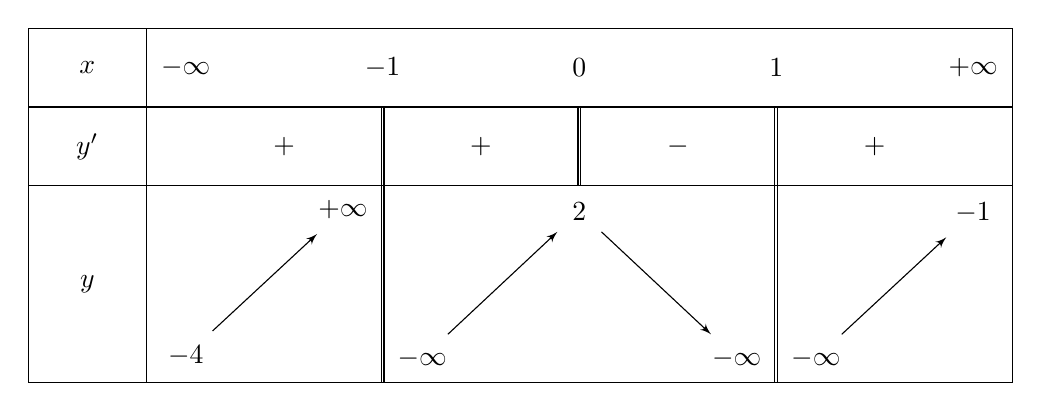
\begin{tikzpicture}
    \tkzTabInit[lgt=1.5, espcl=2.5]
    {$x$ /1, $y'$ /1, $y$ /2.5}
    {$-\infty$, $-1$, $0$, $1$, $+\infty$}
    \tkzTabLine{, +, d, +, d, -, d, +, }
    \tkzTabVar{-/ $-4$ / , +D-/ $+\infty$ /  $-\infty$,+ / $2$ ,  -D-/ $-\infty$ /$-\infty$ , +/ $-1$ /}
\end{tikzpicture}
\end{center}

Tổng số đường tiệm cận ngang và tiệm cận đứng của đồ thị hàm số \( y = f(x) \) là}{
    \begin{tasks}(4)
        \task $3$
        \task $2$
        \task $4$
        \task $1$
    \end{tasks}
}

% --- CÂU 20 ---
\questionLinesManual{0}{20}{Cho hàm số \( y = f(x) \) có bảng biến thiên như hình vẽ dưới đây. Hỏi đồ thị của hàm số đã cho có bao nhiêu đường tiệm cận?

\begin{center}
\begin{tikzpicture}
    \tkzTabInit[lgt=1.5, espcl=2.5]
    {$x$ /1, $y'$ /1, $y$ /2.5}
    {$-\infty$, $-2$, $0$, $+\infty$}
    \tkzTabLine{,,d, +, d, -,}
    \tkzTabVar{,D-// $-\infty$ / , +D+/ $+\infty$ / $1$ , -/ $0$ /}
    \fill[pattern=north east lines](1.5,-4.5) rectangle (4.5,-1);
\end{tikzpicture}
\end{center}

}{
    \begin{tasks}(4)
        \task $3$
        \task $2$
        \task $4$
        \task $1$
    \end{tasks}
}

% --- CÂU 21 ---
\questionLinesManual{0}{21}{Cho hàm số \( y = f(x) \) có bảng biến thiên như sau:

\begin{center}
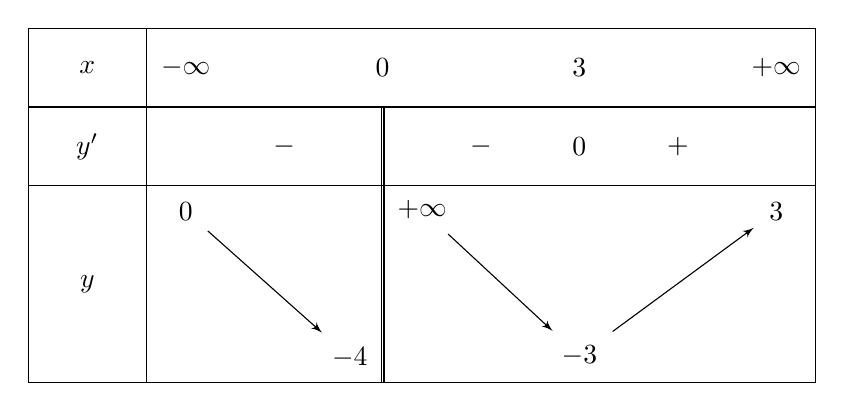
\begin{tikzpicture}
    \tkzTabInit[lgt=1.5, espcl=2.5]
    {$x$ /1, $y'$ /1, $y$ /2.5}
    {$-\infty$, $0$, $3$, $+\infty$}
    \tkzTabLine{, -, d, -, 0, +, }
    \tkzTabVar{+/ $0$ / , -D+/ $-4$ / $+\infty$ , -/ $-3$ / , +/ $3$ /}
\end{tikzpicture}
\end{center}

Tổng số tiệm cận đứng và tiệm cận ngang của đồ thị hàm số đã cho là}{
    \begin{tasks}(4)
        \task $1$
        \task $3$
        \task $4$
        \task $2$
    \end{tasks}
}

% --- CÂU 22 ---
\questionLinesManual{0}{22}{Cho hàm số \( f(x) \) có bảng biến thiên như sau:

\begin{center}
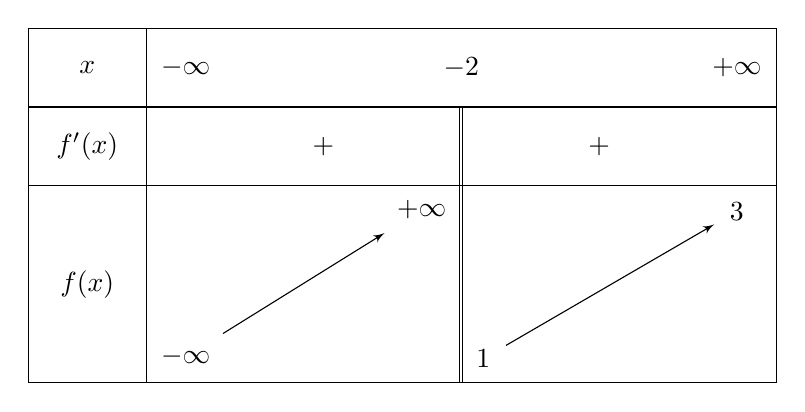
\begin{tikzpicture}
    \tkzTabInit[lgt=1.5, espcl=3.5]
    {$x$ /1, $f'(x)$ /1, $f(x)$ /2.5}
    {$-\infty$, $-2$, $+\infty$}
    \tkzTabLine{, +, d, +, }
    \tkzTabVar{-/ $-\infty$ / , +D-/ $+\infty$ / $1$ , +/ $3$ /}
\end{tikzpicture}
\end{center}

Tổng số tiệm cận ngang và tiệm cận đứng của đồ thị hàm số đã cho là:}{
    \begin{tasks}(4)
        \task $4$
        \task $3$
        \task $1$
        \task $2$
    \end{tasks}
}

% --- CÂU 23 ---
\questionLinesManual{0}{23}{Cho hàm số \( y = f(x) \) có bảng biến thiên như sau:

\begin{center}
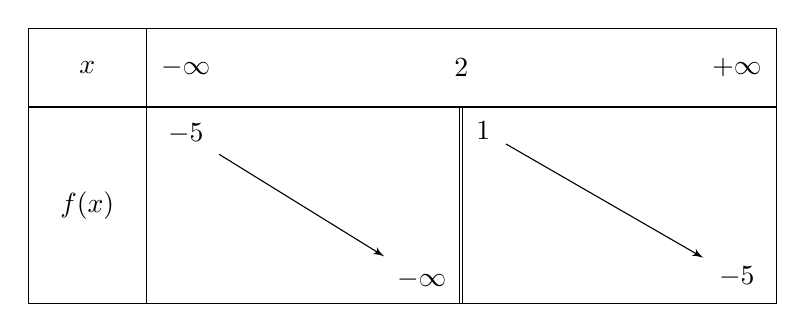
\begin{tikzpicture}
    \tkzTabInit[lgt=1.5, espcl=3.5]
    {$x$ /1, $f(x)$ /2.5}
    {$-\infty$, $2$, $+\infty$}
    \tkzTabVar{+/ $-5$ / , -D+/ $-\infty$ / $1$/ , -/ $-5$ /}
\end{tikzpicture}
\end{center}

Tổng số tiệm cận ngang và tiệm cận đứng của đồ thị hàm số đã cho là:}{
    \begin{tasks}(4)
        \task $4$
        \task $2$
        \task $3$
        \task $1$
    \end{tasks}
}

% --- CÂU 24 ---
\questionLinesManual{0}{24}{Cho hàm số \( f(x) \) có bảng biến thiên như sau

\begin{center}
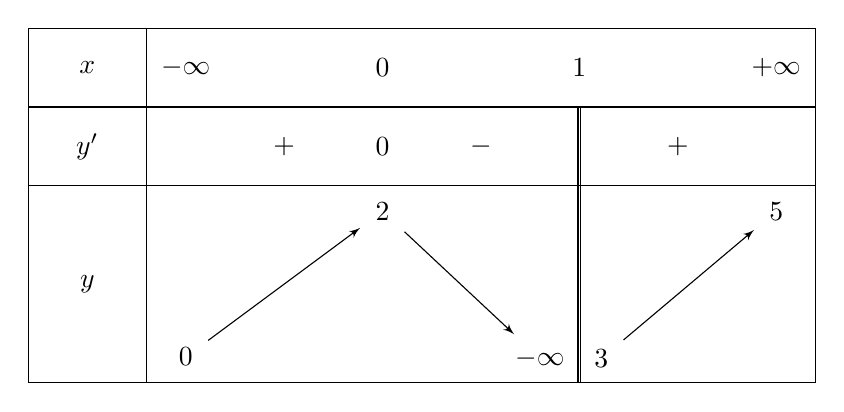
\begin{tikzpicture}
    \tkzTabInit[lgt=1.5, espcl=2.5]
    {$x$ /1, $y'$ /1, $y$ /2.5}
    {$-\infty$, $0$, $1$, $+\infty$}
    \tkzTabLine{, +, 0, -, d, +, }
    \tkzTabVar{-/ $0$ / , +/ $2$ / , -D-/ $-\infty$ / $3$ , +/ $5$ /}
\end{tikzpicture}
\end{center}

Tổng số tiệm cận ngang và tiệm cận đứng của đồ thị hàm số đã cho là}{
    \begin{tasks}(4)
        \task $4$
        \task $1$
        \task $3$
        \task $2$
    \end{tasks}
}

% --- CÂU 25 ---
\questionLinesManual{0}{25}{Cho hàm số \( y = f(x) \) có bảng biến thiên như sau

\begin{center}
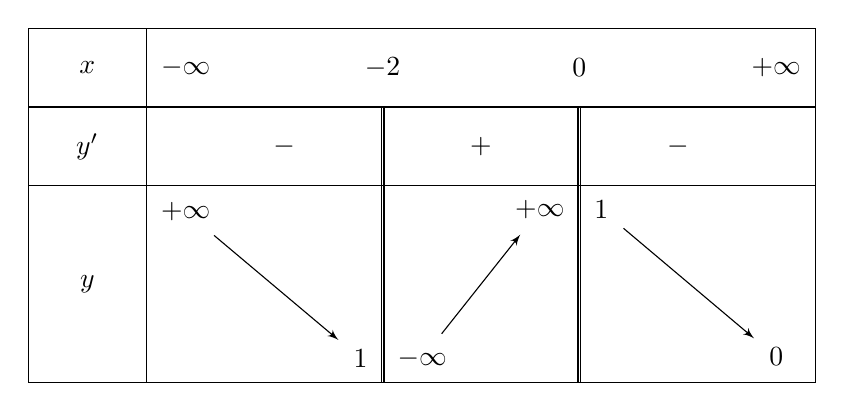
\begin{tikzpicture}
    \tkzTabInit[lgt=1.5, espcl=2.5]
    {$x$ /1, $y'$ /1, $y$ /2.5}
    {$-\infty$, $-2$, $0$, $+\infty$}
    \tkzTabLine{, -, d, +, d, -, }
    \tkzTabVar{+/$+\infty$ / , -D-/ $1$ / $-\infty$,+D+ / $+\infty$ / $1$ , -/ $0$ /}
\end{tikzpicture}
\end{center}

Tổng số đường tiệm cận đứng và tiệm cận ngang của đồ thị hàm số đã cho bằng}{
    \begin{tasks}(4)
        \task $2$
        \task $1$
        \task $0$
        \task $3$
    \end{tasks}
}

% --- CÂU 26 ---
\questionLinesManual{0}{26}{Cho hàm số \( y = f(x) \) liên tục trên \( \mathbb{R} \setminus \{1\} \) có bảng biến thiên như hình vẽ. Tổng số đường tiệm cận đứng và đường tiệm cận ngang của đồ thị hàm số \( y = f(x) \)

\begin{center}
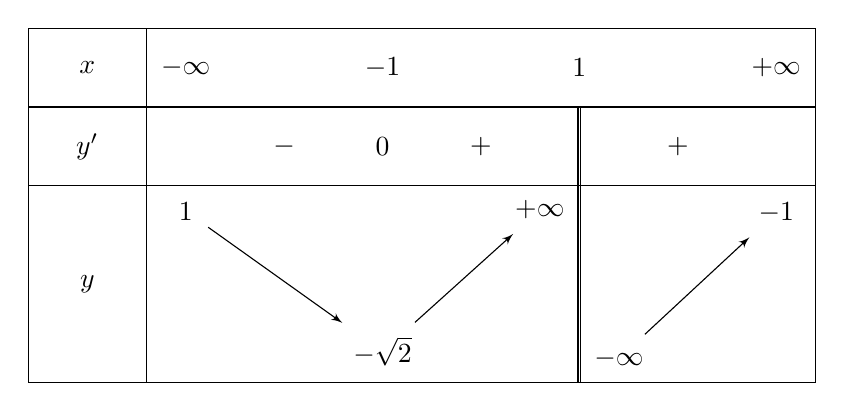
\begin{tikzpicture}
    \tkzTabInit[lgt=1.5, espcl=2.5]
    {$x$ /1, $y'$ /1, $y$ /2.5}
    {$-\infty$, $-1$, $1$, $+\infty$}
    \tkzTabLine{, -, 0, +, d, +, }
    \tkzTabVar{+/$1$/,-/ $-\sqrt{2}$ / ,+D-/ $+\infty$ / $-\infty$ , +/ $-1$ /}
\end{tikzpicture}
\end{center}

}{
    \begin{tasks}(4)
        \task $1$
        \task $4$
        \task $2$
        \task $3$
    \end{tasks}
}

% --- CÂU 27 ---
\questionLinesManual{0}{27}{Cho hàm số \( y = f(x) \) có bảng biến thiên như sau:

\begin{center}
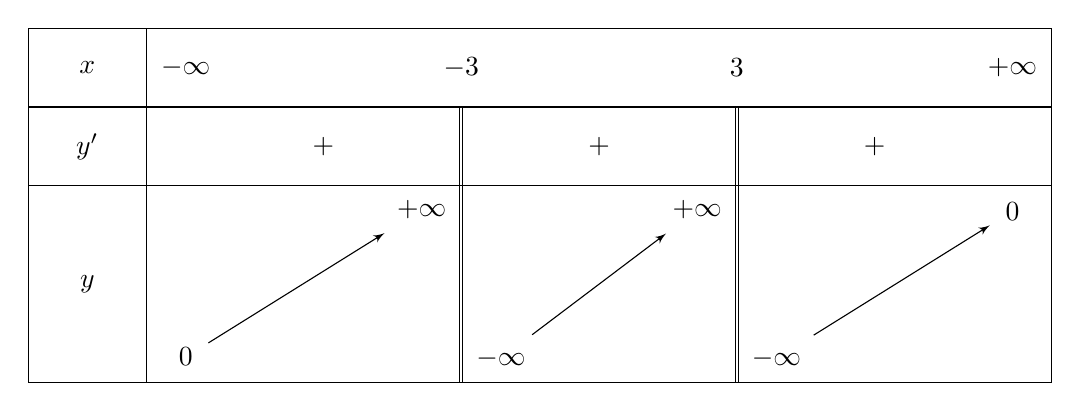
\begin{tikzpicture}
    \tkzTabInit[lgt=1.5, espcl=3.5]
    {$x$ /1, $y'$ /1, $y$ /2.5}
    {$-\infty$, $-3$, $3$, $+\infty$}
    \tkzTabLine{, +, d, +, d, +, }
    \tkzTabVar{-/ $0$ / , +D-/ $+\infty$ / $-\infty$, +D-/ $+\infty$ / $-\infty$, +/ $0$ /}
\end{tikzpicture}
\end{center}

Số đường tiệm cận của đồ thị hàm số là:}{
    \begin{tasks}(4)
        \task $3$
        \task $1$
        \task $4$
        \task $2$
    \end{tasks}
}

% --- CÂU 28 ---
\questionLinesManual{0}{28}{Cho hàm số \( y = f(x) \) có bảng biến thiên như sau:

\begin{center}
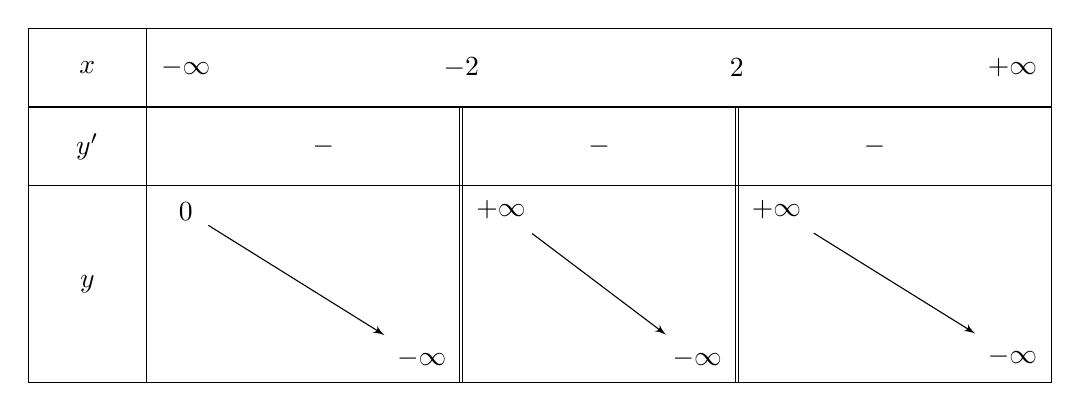
\begin{tikzpicture}
    \tkzTabInit[lgt=1.5, espcl=3.5]
    {$x$ /1, $y'$ /1, $y$ /2.5}
    {$-\infty$, $-2$, $2$, $+\infty$}
    \tkzTabLine{, -, d, -, d, -, }
    \tkzTabVar{+/ $0$ / , -D+/ $-\infty$ / $+\infty$ ,-D+/$-\infty$ / $+\infty$ , -/ $-\infty$ /}
\end{tikzpicture}
\end{center}

Tổng số tiệm cận đứng và tiệm cận ngang của đồ thị hàm số đã cho là}{
    \begin{tasks}(4)
        \task $4$
        \task $2$
        \task $3$
        \task $1$
    \end{tasks}
}

% --- CÂU 29 ---
\questionLinesManual{0}{29}{Cho hàm số \( y = f(x) \) có bảng biến thiên như sau:

\begin{center}
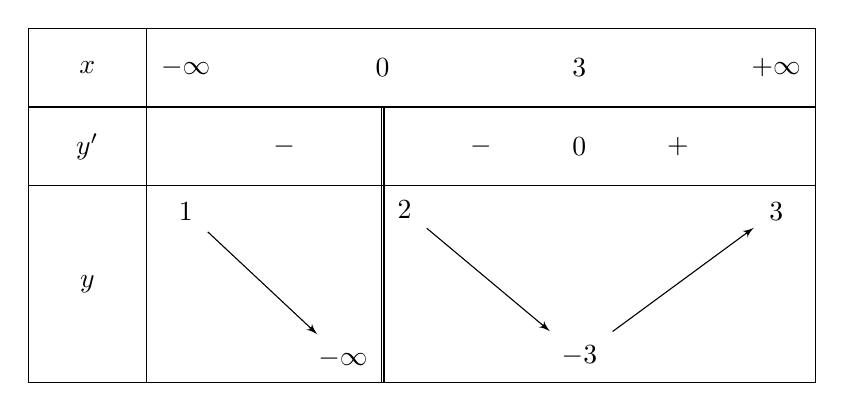
\begin{tikzpicture}
    \tkzTabInit[lgt=1.5, espcl=2.5]
    {$x$ /1, $y'$ /1, $y$ /2.5}
    {$-\infty$, $0$, $3$, $+\infty$}
    \tkzTabLine{, -, d, -, 0, +, }
    \tkzTabVar{+/ $1$ / , -D+/ $-\infty$ / $2$ , -/ $-3$ / , +/ $3$ /}
\end{tikzpicture}
\end{center}

Tổng số tiệm cận đứng và tiệm cận ngang của đồ thị hàm số đã cho là:}{
    \begin{tasks}(4)
        \task $2$
        \task $3$
        \task $4$
        \task $1$
    \end{tasks}
}

% --- CÂU 30 ---
\questionLinesManual{0}{30}{Cho hàm số \( f(x) \) có bảng biến thiên như sau:

\begin{center}
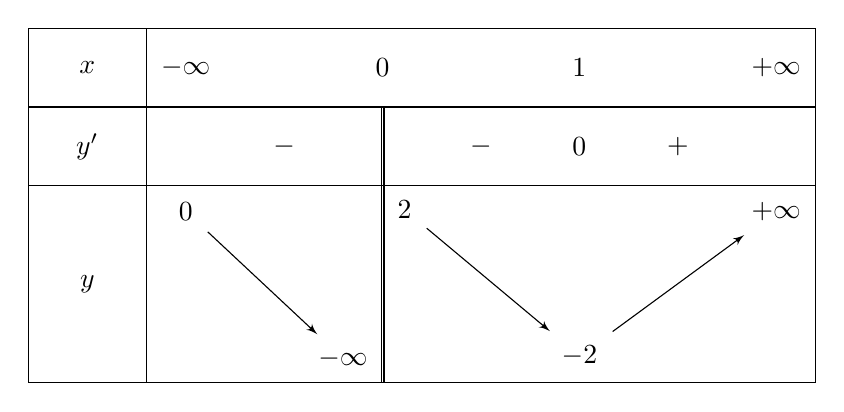
\begin{tikzpicture}
    \tkzTabInit[lgt=1.5, espcl=2.5]
    {$x$ /1, $y'$ /1, $y$ /2.5}
    {$-\infty$, $0$, $1$, $+\infty$}
    \tkzTabLine{, -, d, -, 0, +, }
    \tkzTabVar{+/ $0$ / , -D+/ $-\infty$ / $2$ , -/ $-2$ / , +/ $+\infty$ /}
\end{tikzpicture}
\end{center}

Tổng số tiệm cận đứng và tiệm cận ngang của đồ thị hàm số đã cho là:}{
    \begin{tasks}(4)
        \task $1$
        \task $2$
        \task $4$
        \task $3$
    \end{tasks}
}

% --- CÂU 31 ---
\questionLinesManual{0}{31}{Cho hàm số \( y = f(x) \) có bảng biến thiên như sau:

\begin{center}
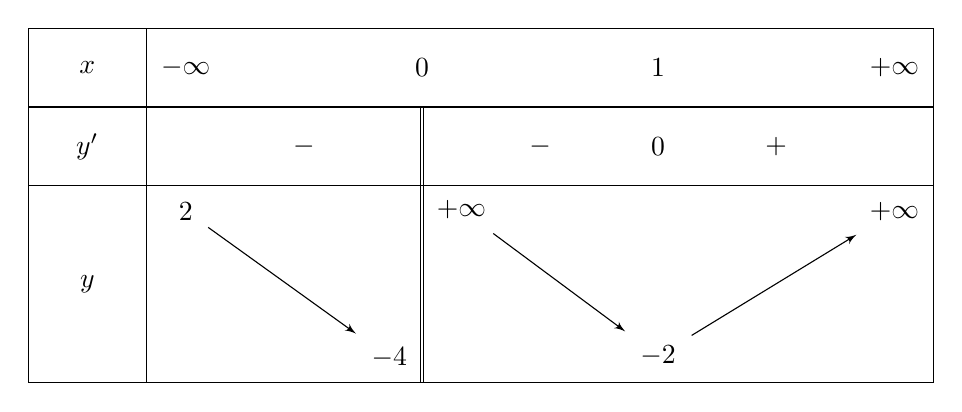
\begin{tikzpicture}
    \tkzTabInit[lgt=1.5, espcl=3]
    {$x$ /1, $y'$ /1, $y$ /2.5}
    {$-\infty$, $0$, $1$, $+\infty$}
    \tkzTabLine{, -, d, -, 0, +, }
    \tkzTabVar{+/ $2$ / , -D+/ $-4$ / $+\infty$ , -/ $-2$ / , +/ $+\infty$ /}
\end{tikzpicture}
\end{center}

Tổng số tiệm cận đứng và tiệm cận ngang của đồ thị hàm số đã cho là:}{
    \begin{tasks}(4)
        \task $4$
        \task $1$
        \task $3$
        \task $2$
    \end{tasks}
}

% --- CÂU 32 ---
\questionLinesManual{0}{32}{Cho hàm số \( y = f(x) \) có bảng biến thiên như sau

\begin{center}
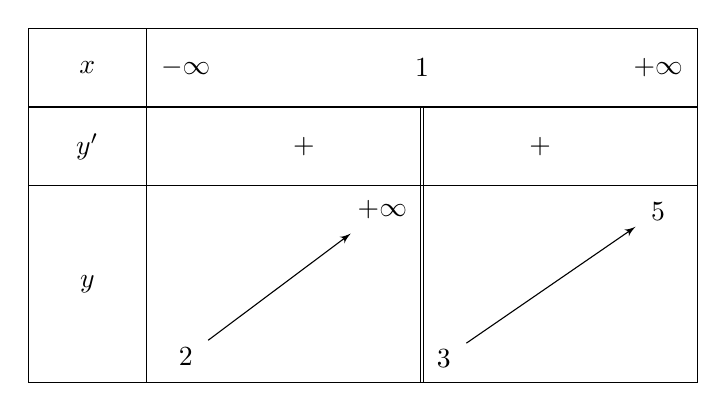
\begin{tikzpicture}
    \tkzTabInit[lgt=1.5, espcl=3]
    {$x$ /1, $y'$ /1, $y$ /2.5}
    {$-\infty$, $1$, $+\infty$}
    \tkzTabLine{, +, d, +, }
    \tkzTabVar{-/ $2$ / , +D-/ $+\infty$ / $3$ , +/ $5$ /}
\end{tikzpicture}
\end{center}

Tổng số đường tiệm cận ngang và đường tiệm cận đứng của đồ thị hàm số đã cho là}{
    \begin{tasks}(4)
        \task $3$
        \task $2$
        \task $4$
        \task $1$
    \end{tasks}
}

% --- CÂU 33 ---
\questionLinesManual{0}{33}{Cho hàm số có bảng biến thiên như hình sau

\begin{center}
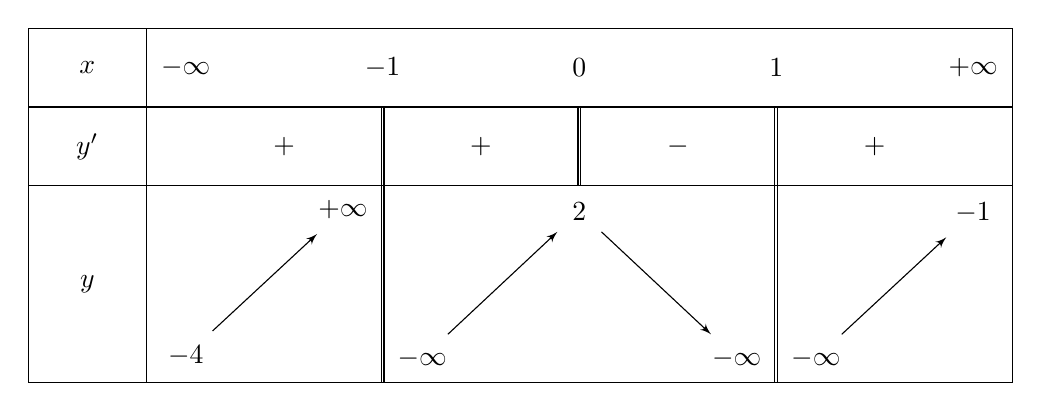
\begin{tikzpicture}
    \tkzTabInit[lgt=1.5, espcl=2.5]
    {$x$ /1, $y'$ /1, $y$ /2.5}
    {$-\infty$, $-1$, $0$, $1$, $+\infty$}
    \tkzTabLine{, +, d, +, d, -, d, +, }
    \tkzTabVar{-/ $-4$ / , +D-/ $+\infty$ / $-\infty$ , +/ $2$ / , -D-/ $-\infty$ /$-\infty$ / , +/ $-1$ /}
\end{tikzpicture}
\end{center}

Tổng số đường tiệm cận ngang và tiệm cận đứng của đồ thị hàm số \( y = f(x) \) là}{
    \begin{tasks}(4)
        \task $3$
        \task $2$
        \task $4$
        \task $1$
    \end{tasks}
}

% --- CÂU 34 ---
\questionLinesManual{0}{34}{Cho hàm số \( y = f(x) \) có bảng biến thiên như hình vẽ dưới đây. Hỏi đồ thị của hàm số đã cho có bao nhiêu đường tiệm cận?

\begin{center}
\begin{tikzpicture}
    \tkzTabInit[lgt=1.5, espcl=3.5]
    {$x$ /1, $y'$ /1, $y$ /2.5}
    {$-\infty$, $-2$, $0$, $+\infty$}
    \tkzTabLine{,,d, +, d, -, }
    \tkzTabVar{,D-/ /$-\infty$ / , +D+/ $+\infty$ / $1$ , -/ $0$ /}
    \fill[pattern=north east lines](1.5,-4.5) rectangle (5.5,-1);
\end{tikzpicture}
\end{center}

}{
    \begin{tasks}(4)
        \task $3$
        \task $2$
        \task $4$
        \task $1$
    \end{tasks}
}

% --- CÂU 35 ---
\questionLinesManual{0}{35}{Cho hàm số \( y = f(x) \) có bảng biến thiên như sau:

\begin{center}
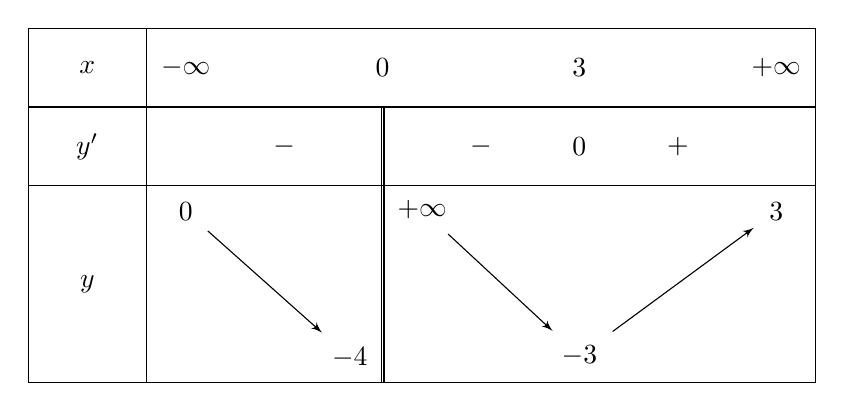
\begin{tikzpicture}
    \tkzTabInit[lgt=1.5, espcl=2.5]
    {$x$ /1, $y'$ /1, $y$ /2.5}
    {$-\infty$, $0$, $3$, $+\infty$}
    \tkzTabLine{, -, d, -, 0, +, }
    \tkzTabVar{+/ $0$ / , -D+/ $-4$ / $+\infty$ , -/ $-3$ / , +/ $3$ /}
\end{tikzpicture}
\end{center}

Tổng số tiệm cận đứng và tiệm cận ngang của đồ thị hàm số đã cho là}{
    \begin{tasks}(4)
        \task $1$
        \task $3$
        \task $4$
        \task $2$
    \end{tasks}
}

% --- CÂU 36 ---
\questionLinesManual{0}{36}{Cho hàm số \( f(x) \) có bảng biến thiên như sau:

\begin{center}
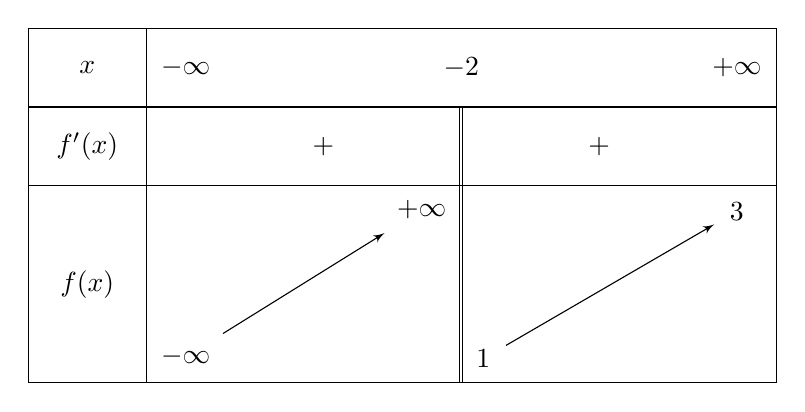
\begin{tikzpicture}
    \tkzTabInit[lgt=1.5, espcl=3.5]
    {$x$ /1, $f'(x)$ /1, $f(x)$ /2.5}
    {$-\infty$, $-2$, $+\infty$}
    \tkzTabLine{, +, d, +, }
    \tkzTabVar{-/ $-\infty$ / , +D-/ $+\infty$ / $1$ , +/ $3$ /}
\end{tikzpicture}
\end{center}

Tổng số tiệm cận ngang và tiệm cận đứng của đồ thị hàm số đã cho là:}{
    \begin{tasks}(4)
        \task $4$
        \task $3$
        \task $1$
        \task $2$
    \end{tasks}
}

% --- CÂU 37 ---
\questionLinesManual{0}{37}{Cho hàm số \( y = f(x) \) có bảng biến thiên như sau:

\begin{center}
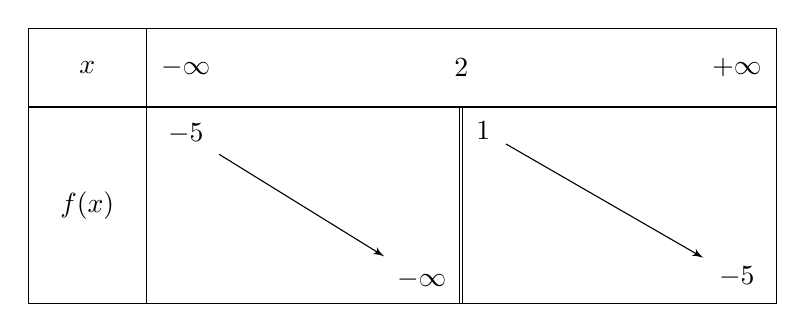
\begin{tikzpicture}
    \tkzTabInit[lgt=1.5, espcl=3.5]
    {$x$ /1,  $f(x)$ /2.5}
    {$-\infty$, $2$, $+\infty$}
    \tkzTabVar{+/ $-5$ / , -D+/ $-\infty$ / $1$/ , -/ $-5$ /}
\end{tikzpicture}
\end{center}

Tổng số tiệm cận ngang và tiệm cận đứng của đồ thị hàm số đã cho là:}{
    \begin{tasks}(4)
        \task $4$
        \task $2$
        \task $3$
        \task $1$
    \end{tasks}
}

% --- CÂU 38 ---
\questionLinesManual{0}{38}{Cho hàm số \( f(x) \) có bảng biến thiên như sau

\begin{center}
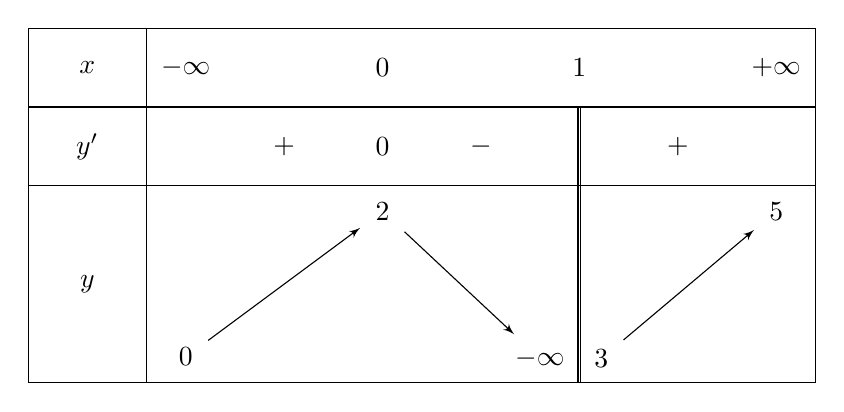
\begin{tikzpicture}
    \tkzTabInit[lgt=1.5, espcl=2.5]
    {$x$ /1, $y'$ /1, $y$ /2.5}
    {$-\infty$, $0$, $1$, $+\infty$}
    \tkzTabLine{, +, 0, -, d, +, }
    \tkzTabVar{-/ $0$ / , +/ $2$ / , -D-/ $-\infty$ / $3$ , +/ $5$ /}
\end{tikzpicture}
\end{center}

Tổng số tiệm cận ngang và tiệm cận đứng của đồ thị hàm số đã cho là}{
    \begin{tasks}(4)
        \task $4$
        \task $1$
        \task $3$
        \task $2$
    \end{tasks}
}

% --- CÂU 39 ---
\questionLinesManual{0}{39}{Cho hàm số \( y = f(x) \) có bảng biến thiên như sau

\begin{center}
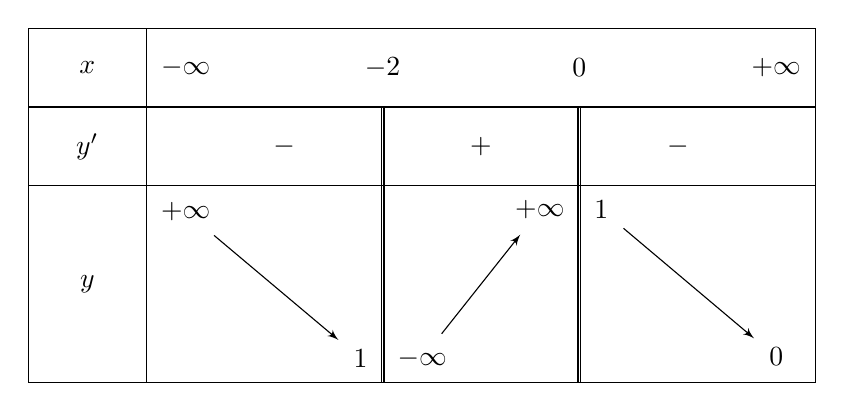
\begin{tikzpicture}
    \tkzTabInit[lgt=1.5, espcl=2.5]
    {$x$ /1, $y'$ /1, $y$ /2.5}
    {$-\infty$, $-2$, $0$, $+\infty$}
    \tkzTabLine{, -, d, +, d, -, }
    \tkzTabVar{+/ $+\infty$ / ,-D-/ $1$/$-\infty$ , +D+/ $+\infty$ / $1$ , -/ $0$ /}
\end{tikzpicture}
\end{center}

Tổng số đường tiệm cận đứng và tiệm cận ngang của đồ thị hàm số đã cho bằng}{
    \begin{tasks}(4)
        \task $2$
        \task $1$
        \task $0$
        \task $3$
    \end{tasks}
}

% --- CÂU 40 ---
\questionLinesManual{0}{40}{Cho hàm số \( y = f(x) \) liên tục trên \( \mathbb{R} \setminus \{1\} \) có bảng biến thiên như hình vẽ. Tổng số đường tiệm cận đứng và đường tiệm cận ngang của đồ thị hàm số \( y = f(x) \)

\begin{center}
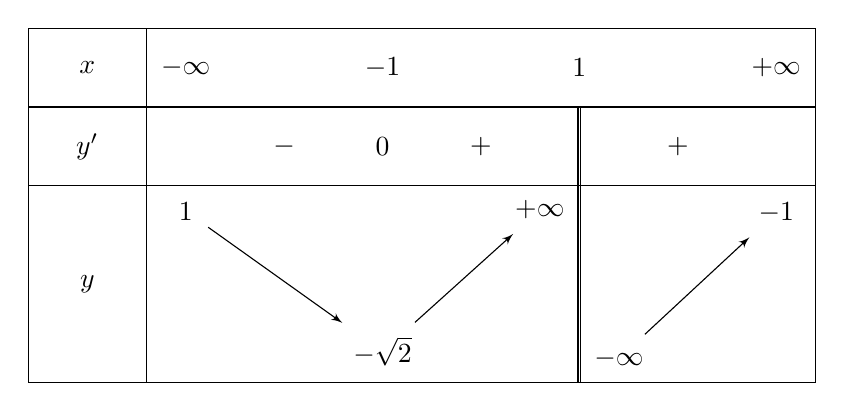
\begin{tikzpicture}
    \tkzTabInit[lgt=1.5, espcl=2.5]
    {$x$ /1, $y'$ /1, $y$ /2.5}
    {$-\infty$, $-1$, $1$, $+\infty$}
    \tkzTabLine{, -, 0, +, d, +, }
    \tkzTabVar{ +/ $1$ / ,-/ $-\sqrt{2}$ /, +D-/ $+\infty$ / $-\infty$ , +/ $-1$ /}
\end{tikzpicture}
\end{center}

}{
    \begin{tasks}(4)
        \task $1$
        \task $4$
        \task $2$
        \task $3$
    \end{tasks}
}

% --- CÂU 41 ---
\questionLinesManual{0}{41}{Cho hàm số \( y = f(x) \) có bảng biến thiên như sau:

\begin{center}
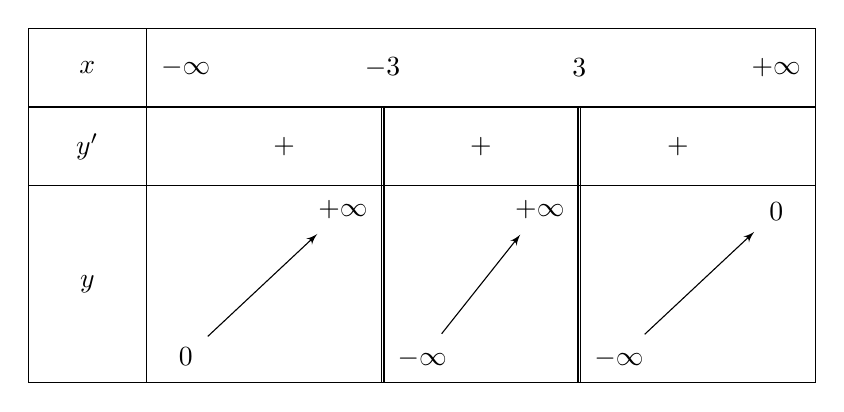
\begin{tikzpicture}
    \tkzTabInit[lgt=1.5, espcl=2.5]
    {$x$ /1, $y'$ /1, $y$ /2.5}
    {$-\infty$, $-3$, $3$, $+\infty$}
    \tkzTabLine{, +, d, +, d, +, }
    \tkzTabVar{-/ $0$ / , +D-/ $+\infty$ / $-\infty$, +D-/ $+\infty$ / $-\infty$, +/ $0$ /}
\end{tikzpicture}
\end{center}

Số đường tiệm cận của đồ thị hàm số là:}{
    \begin{tasks}(4)
        \task $3$
        \task $1$
        \task $4$
        \task $2$
    \end{tasks}
}

% --- CÂU 42 ---
\questionLinesManual{0}{42}{Cho hàm số \( y = f(x) \) có bảng biến thiên như sau:

\begin{center}
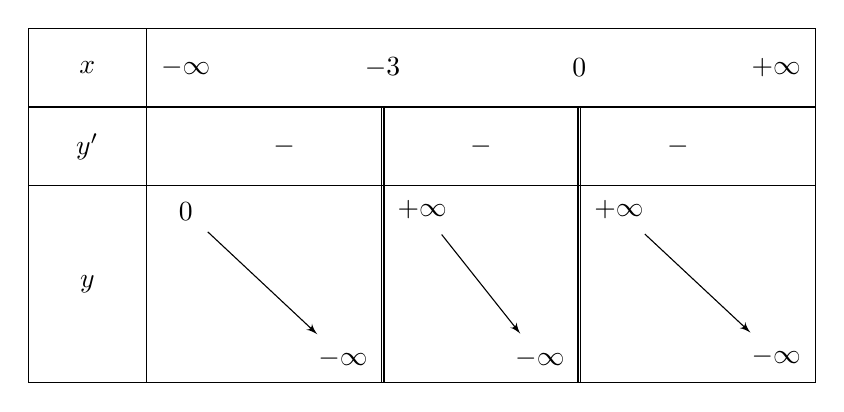
\begin{tikzpicture}
    \tkzTabInit[lgt=1.5, espcl=2.5]
    {$x$ /1, $y'$ /1, $y$ /2.5}
    {$-\infty$, $-3$, $0$, $+\infty$}
    \tkzTabLine{, -, d, -, d, -, }
    \tkzTabVar{+/ $0$ / , -D+/ $-\infty$ / $+\infty$ ,-D+/ $-\infty$ / $+\infty$  , -/ $-\infty$ /}
\end{tikzpicture}
\end{center}

Tổng số tiệm cận đứng và tiệm cận ngang của đồ thị hàm số đã cho là}{
    \begin{tasks}(4)
        \task $4$
        \task $2$
        \task $3$
        \task $1$
    \end{tasks}
}

\questionLinesManual{0}{43}{Cho hàm số \( y = f(x) \) có bảng biến thiên như sau

\begin{center}
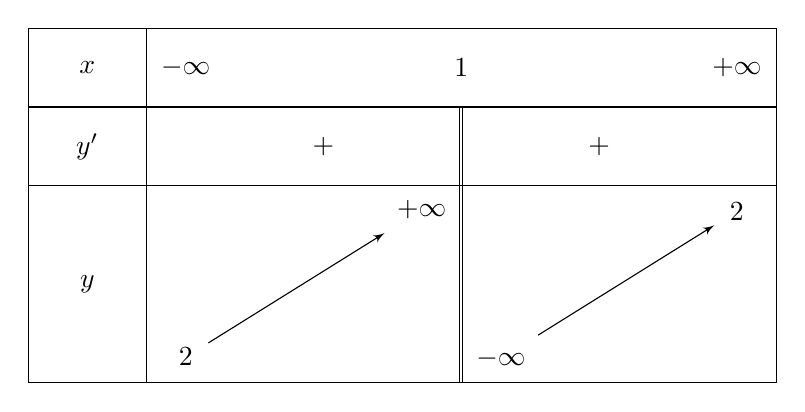
\begin{tikzpicture}
    \tkzTabInit[lgt=1.5, espcl=3.5]
    {$x$ /1, $y'$ /1, $y$ /2.5}
    {$-\infty$, $1$, $+\infty$}
    \tkzTabLine{, +, d, +, }
    \tkzTabVar{-/ $2$ / , +D-/ $+\infty$ / $-\infty$, +/ $2$ /}
\end{tikzpicture}
\end{center}

Tổng số tiệm cận ngang và tiệm cận đứng của đồ thị hàm số đã cho là}{
    \begin{tasks}(4)
        \task $4$
        \task $1$
        \task $3$
        \task $2$
    \end{tasks}
}

% --- CÂU 44 ---
\questionLinesManual{0}{44}{Cho hàm số \( y = f(x) \) có đồ thị như hình vẽ. Đường thẳng nào sau đây là tiệm cận ngang của đồ thị hàm số đã cho

\begin{center}
\begin{tikzpicture}[>=latex, scale=1]
    % 1. Hệ trục tọa độ
    \draw[->] (-4.5,0) -- (3.5,0) node[below] {\small $x$};
    \draw[->] (0,-4.5) -- (0,3.5) node[right] {\small $y$};
    \node[below left] at (0,0) {\small $O$};
    
    % 2. Vẽ đồ thị hàm số
    \draw[thick, samples=100, domain=-4.5:-1.45] 
        plot (\x, {(-\x+0.5)/(\x + 1)});
    \draw[thick, samples=100, domain=-0.65:3.5] 
         plot (\x, {(-\x+0.5)/(\x + 1)});
    
    % 3. Đường tiệm cận
    \draw[thick] (-1,-4.5) -- (-1,3.5);
    \draw[thick] (-4.5,-1) -- (3.5,-1) ;
    % 4. Đánh dấu các điểm
    \node[below left] at (0,-1) {\small $-1$};
    \node[below left] at (-1,0) {\small $-1$};
\end{tikzpicture}
\end{center}

}{
    \begin{tasks}(4)
        \task \( x = 1 \)
        \task \( x = -1 \)
        \task \( y = 1 \)
        \task \( y = -1 \)
    \end{tasks}
}

% --- CÂU 45 ---
\questionLinesManual{0}{45}{Cho hàm số \( y = \dfrac{ax + b}{cx + d} \) (\( c \neq 0 \), \( ad - bc \neq 0 \)) có đồ thị như hình vẽ bên. Tiệm cận ngang của đồ thị hàm số là:

\begin{center}
\begin{tikzpicture}[>=latex, scale=1]
    % 1. Hệ trục tọa độ
    \draw[->] (-3.5,0) -- (3.5,0) node[below] {\small $x$};
    \draw[->] (0,-3.5) -- (0,3.5) node[right] {\small $y$};
    \node[below left] at (0,0) {\small $O$};
    
    % 2. Vẽ đồ thị hàm số
    \draw[thick, samples=100, domain=-3.5:-1.13] 
        plot (\x, {0.5 + 0.5/(\x + 1)});
    \draw[thick, samples=100, domain=-0.83:3.5] 
        plot (\x, {0.5 + 0.5/(\x + 1)});
    
    % 3. Đường tiệm cận
    \draw[thick] (-1,-3.5) -- (-1,3.5) ;
    \draw[thick] (-3.5,0.5) -- (3.5,0.5) ;
    
    % 4. Đánh dấu các điểm
    \node[above left] at (0,0.5) {\small $\frac{1}{2}$};
    \node[below left] at (-1,0) {\small $-1$};
\end{tikzpicture}
\end{center}

}{
    \begin{tasks}(4)
        \task \( x = -1 \)
        \task \( y = \dfrac{1}{2} \)
        \task \( y = -1 \)
        \task \( x = \dfrac{1}{2} \)
    \end{tasks}
}

% --- CÂU 46 ---
\questionLinesManual{0}{46}{Hàm số \( y = \dfrac{ax + b}{cx + d} \) (\( c \neq 0 \), \( ad - bc \neq 0 \)) có đồ thị dưới đây. Đường tiệm cận đứng của đồ thị hàm số là:

\begin{center}
\begin{tikzpicture}[>=latex, scale=1]
    % 1. Hệ trục tọa độ
    \draw[->] (-3.5,0) -- (6.5,0) node[below] {\small $x$};
    \draw[->] (0,-3.5) -- (0,4.5) node[right] {\small $y$};
    \node[below left] at (0,0) {\small $O$};
    
    % 2. Vẽ đồ thị hàm số
    \draw[thick, samples=100, domain=-3.5:1.81] 
        plot (\x, {(-\x+1)/(\x -2) });
    \draw[thick, samples=100, domain=2.39:6.5] 
         plot (\x, {(-\x+1)/(\x -2) });
    
    % 3. Đường tiệm cận
    \draw[dashed] (2,-3.5) -- (2,4.5) ;
    \draw[dashed] (-3.5,-1) -- (6.5,-1) ;
    
    % 4. Đánh dấu các điểm
    \node[ below left] at (0,-1) {\small $-1$};
    \node[below right] at (1,0) {\small $1$};
    \node[below right] at (2,0) {\small $2$};
    \filldraw (2,0) circle (1.5pt);
    \filldraw (1,0) circle (1.5pt);
    \filldraw (0,-1) circle (1.5pt);
\end{tikzpicture}
\end{center}

}{
    \begin{tasks}(4)
        \task \( x = -1 \)
        \task \( x = 1 \)
        \task \( x = 2 \)
        \task \( y = -1 \)
    \end{tasks}
}

% --- CÂU 47 ---
\questionLinesManual{0}{47}{Cho hàm số \( y = f(x) \) có đồ thị như hình vẽ:

\begin{center}
\begin{tikzpicture}[>=latex, scale=0.7]
    % 1. Hệ trục tọa độ
    \draw[->] (-3.5,0) -- (7.5,0) node[below] {\small $x$};
    \draw[->] (0,-4.5) -- (0,5) node[right] {\small $y$};
    \node[below left] at (0,0) {\small $O$};
    
    % 2. Vẽ đồ thị hàm số
    \draw[thick, samples=100, domain=-3:0.65] 
        plot (\x, {-\x+2 + 2/(\x -1)});
    \draw[thick, samples=100, domain=1.45:6.5] 
        plot (\x, {-\x+2 + 2/(\x -1)});
    \draw[thick, samples=100, domain=-3:6] 
        plot (\x, {-\x+2 });
    % 3. Đường tiệm cận
    \draw[thick] (1,-4.5) -- (1,5) ;
   
    
    % 4. Đánh dấu các điểm
    \node[left] at (0,-2) {\small $-2$};
     \node[left] at (0,2) {\small $2$};
    \node[below] at (-2,0) {\small $-2$};
    \node[below] at (2,0) {\small $2$};
    \node[below] at (4,0) {\small $4$};
    \node[below] at (6,0) {\small $6$};
\end{tikzpicture}
\end{center}

Đồ thị hàm số đã cho có bao nhiêu đường tiệm cận?}{
    \begin{tasks}(4)
        \task $4$
        \task $1$
        \task $3$
        \task $2$
    \end{tasks}
}

% --- CÂU 48 ---
\questionLinesManual{0}{48}{Cho hàm số \( y = \dfrac{ax^2 + bx + c}{mx + n} \) (với \( a \neq 0; m \neq 0 \)) có đồ thị như hình vẽ dưới đây.

\begin{center}
\begin{tikzpicture}[>=latex, scale=0.8]
    % 1. Hệ trục tọa độ
    \draw[->] (-3.5,0) -- (5.5,0) node[below] {\small $x$};
    \draw[->] (0,-4.5) -- (0,4.5) node[right] {\small $y$};
    \node[below left] at (0,0) {\small $O$};
    
    % 2. Vẽ đồ thị hàm số
    \draw[thick, samples=100, domain=-2.5:1.75] 
        plot (\x, {\x-2 + 1/(\x -2)});
    \draw[thick, samples=100, domain=2.25:5] 
        plot (\x, {\x-2 + 1/(\x -2)});
    \draw[thick, samples=100, domain=-2.5:5] 
        plot (\x, {\x-2});
    
    % 4. Đường tiệm cận đứng
    \draw[thick] (2,-4.5) -- (2,4.5) ;
    
    % 5. Đánh dấu các điểm
    \node[above left] at (1,0) {\small $1$};
     \node[above left] at (2,0) {\small $2$};
      \node[above left] at (0,-2) {\small $-2$};
    \draw [dashed] (1,0) -- (1,-2) -- (0,-2);
\end{tikzpicture}
\end{center}

Phương trình đường tiệm cận xiên của đồ thị hàm số đã cho là:}{
    \begin{tasks}(4)
        \task \( y = 2x + 2 \)
        \task \( y = x - 2 \)
        \task \( y = 2x - 2 \)
        \task \( y = x + 2 \)
    \end{tasks}
}

% --- CÂU 49 ---
\questionLinesManual{0}{49}{Cho hàm số \( y = \dfrac{ax + b}{cx + d} \) (\( c \neq 0, ad - bc \neq 0 \)) có đồ thị như hình vẽ bên. Tiệm cận đứng của đồ thị hàm số là:

\begin{center}
\begin{tikzpicture}[>=latex, scale=0.8]
    % 1. Hệ trục tọa độ
    \draw[->] (-3.5,0) -- (5.5,0) node[below] {\small $x$};
    \draw[->] (0,-4.5) -- (0,3.5) node[right] {\small $y$};
    \node[below left] at (0,0) {\small $O$};
    
    % 2. Vẽ đồ thị hàm số
    \draw[thick, samples=100, domain=-3.5:0.71] 
        plot (\x, {(-\x+2)/(\x - 1)});
    \draw[thick, samples=100, domain=1.22:5] 
        plot (\x, {(-\x+2)/(\x - 1)});
    % 3. Đường tiệm cận
    \draw[thick] (1,-4.5) -- (1,3.5);
    \draw[thick] (-3.5,-1) -- (3.5,-1) ;
    
    % 4. Đánh dấu các điểm
    \node[below left] at (1,0) {\small $1$};
    \node[below left] at (2,0) {\small $2$};
    \node[below left ] at (0,-1) {\small $-1$};
    \node[below left] at (0,-2) {\small $-2$};
    \filldraw (1,-2) circle (1.5pt);
    \filldraw (2,0) circle (1.5pt);
    \filldraw (0,-1) circle (1.5pt);
    \filldraw (0,-2) circle (1.5pt);
\end{tikzpicture}
\end{center}

}{
    \begin{tasks}(4)
        \task \( x = -1 \)
        \task \( y = -1 \)
        \task \( x = 1 \)
        \task \( y = 1 \)
    \end{tasks}
}

% --- CÂU 50 ---
\questionLinesManual{0}{50}{Cho hàm số \( y = \dfrac{ax^2 + bx + c}{x} \), (\(ac \neq 0\)) có đồ thị như hình vẽ. Đường tiệm cận xiên của đồ thị hàm số đã cho là đường thẳng có phương trình

\begin{center}
\begin{tikzpicture}[>=latex, scale=0.4]
    % 1. Hệ trục tọa độ
    \draw[->] (-7.5,0) -- (7.5,0) node[below] {\small $x$};
    \draw[->] (0,-9) -- (0,9) node[right] {\small $y$};
    \node[below left] at (0,0) {\small $O$};
    
    % 2. Vẽ đồ thị hàm số
    \draw[thick, samples=100, domain=-6:-0.46] 
        plot (\x, {-\x - 4/(\x)});
    \draw[thick, samples=100, domain=0.46:6] 
        plot (\x, {-\x - 4/(\x)});
     \draw[thick, samples=100, domain=-6:4.6] 
        plot (\x, {-\x });
    \draw[dashed] (-2,0) -- (-2,4)-- (0,4);
    \draw[dashed] (2,0) -- (2,-4)-- (0,-4);
    % 5. Đánh dấu các điểm
    \node[below] at (-2,0) {\small $-2$};
    \node[below] at (2,0) {\small $2$};
    \node[left] at (0,4) {\small $4$};
    \node[left] at (0,-4) {\small $-4$};
    \filldraw (-2,0) circle (1.5pt);
    \filldraw (2,0) circle (1.5pt);
    \filldraw (0,4) circle (1.5pt);
    \filldraw (0,-4) circle (1.5pt);
\end{tikzpicture}
\end{center}

}{
    \begin{tasks}(4)
        \task \( y = x \)
        \task \( y = -x \)
        \task \( x = 0 \)
        \task \( y = 2x \)
    \end{tasks}
}

% --- CÂU 51 ---
\questionLinesManual{0}{51}{Cho hàm số \( y = \dfrac{ax + b}{cx + d} \) (\( c \neq 0; ad - bc \neq 0 \)) có đồ thị như hình vẽ.

\begin{center}
\begin{tikzpicture}[>=latex, scale=0.6]
    % 1. Hệ trục tọa độ
    \draw[->] (-6.5,0) -- (6.5,0) node[below] {\small $x$};
    \draw[->] (0,-4.5) -- (0,6.5) node[right] {\small $y$};
    \node[below left] at (0,0) {\small $O$};
    
    % 2. Vẽ đồ thị hàm số
    \draw[thick, samples=100, domain=-6.5:-1.65] 
        plot (\x, {(2*\x - 1)/(\x +1)});
    \draw[thick, samples=100, domain=-0.54:6.6] 
        plot (\x, {(2*\x - 1)/(\x +1)});
    % 3. Đường tiệm cận
    \draw[thick] (-1,-4.5) -- (-1,6.5) ;
    \draw[thick] (-6.5,2) -- (6.5,2);
    
    % 4. Đánh dấu các điểm
    \node[right] at (0,-1) {\small $-1$};
    \node[above right] at (0,2) {\small $2$};
    \node[below left] at (-1,0) {\small $-1$};
    \filldraw (-1,0) circle (1.5pt);
    \filldraw (0,2) circle (1.5pt);
    \filldraw (0,-1) circle (1.5pt);
\end{tikzpicture}
\end{center}

Tiệm cận ngang của đồ thị hàm số đã cho là}{
    \begin{tasks}(4)
        \task \( x = 2 \)
        \task \( y = 1 \)
        \task \( y = 2 \)
        \task \( x = 2 \)
    \end{tasks}
}

% --- CÂU 52 ---
\questionLinesManual{0}{52}{Cho hàm số \( y = \dfrac{ax^2 + bx + c}{mx + n} \) có đồ thị như hình bên.

\begin{center}
\begin{tikzpicture}[>=latex, scale=1]
    % 1. Hệ trục tọa độ
    \draw[->] (-4.5,0) -- (4.5,0) node[below] {\small $x$};
    \draw[->] (0,-4.5) -- (0,4.5) node[right] {\small $y$};
    \node[below left] at (0,0) {\small $O$};
    
    % 2. Vẽ đồ thị hàm số
    \draw[thick, samples=100, domain=-4:-1.25] 
        plot (\x, {-\x - 1 + -1/(\x + 1)});
     \draw[thick, samples=100, domain=-0.75:3] 
        plot (\x, {-\x - 1 + -1/(\x + 1)});
     \draw[thick, samples=100, domain=-4:3] 
        plot (\x, {-\x - 1});
    \draw[thick] (-1,-4.5) -- (-1,4.5) ;
    
    % 5. Đánh dấu các điểm
    \node[below left] at (-1,0) {\small $-1$};
    \node[below] at (1,0) {\small $1$};
    \node[below left] at (0,-1) {\small $-1$};
    \filldraw (-1,0) circle (1.5pt);
    \filldraw (1,0) circle (1.5pt);
    \filldraw (0,-1) circle (1.5pt);
\end{tikzpicture}
\end{center}

Tiệm cận xiên của đồ thị hàm số đã cho là}{
    \begin{tasks}(4)
        \task \( y = -x + 1 \)
        \task \( y = x - 1 \)
        \task \( y = -x - 1 \)
        \task \( y = x + 1 \)
    \end{tasks}
}

% --- CÂU 53 ---
\questionLinesManual{0}{53}{Cho hàm số \( y = \dfrac{ax + b}{cx + d} \) (\( c \neq 0; ad - bc \neq 0 \)) có đồ thị như hình vẽ bên dưới.

\begin{center}
\begin{tikzpicture}[>=latex, scale=1]
    % 1. Hệ trục tọa độ
    \draw[->] (-3.5,0) -- (5.5,0) node[below] {\small $x$};
    \draw[->] (0,-3.5) -- (0,2.5) node[right] {\small $y$};
    \node[below left] at (0,0) {\small $O$};
    
    % 2. Vẽ đồ thị hàm số
    \draw[thick, samples=100, domain=-3.5:0.6] 
        plot (\x, {(-\x+2)/(\x - 1)});
    \draw[thick, samples=100, domain=1.3:5.5] 
        plot (\x, {(-\x+2)/(\x - 1)});
    
    % 3. Đường tiệm cận
    \draw[thick] (1,-3.5) -- (1,2.5);
    \draw[thick] (-3.5,-1) -- (5.5,-1);
    
    % 4. Đánh dấu các điểm
    \node[ below left] at (0,-1) {\small $-1$};
    \node[below left] at (1,0) {\small $1$};
     \node[below] at (2,0) {\small $2$};
      \node[below] at (0,-2) {\small $-2$};
    \filldraw (1,0) circle (1.5pt);
    \filldraw (2,0) circle (1.5pt);
    \filldraw (0,-1) circle (1.5pt);
    \filldraw (0,-2) circle (1.5pt);
\end{tikzpicture}
\end{center}

Đồ thị hàm số có đường tiệm cận ngang là:}{
    \begin{tasks}(4)
        \task \( y = 0 \)
        \task \( y = -1 \)
        \task \( x = -1 \)
        \task \( y = 1 \)
    \end{tasks}
}

% --- CÂU 54 ---
\questionLinesManual{0}{54}{Đồ thị dưới đây là của hàm số nào trong các hàm số cho ở các phương án \( A, B, C, D \)?

\begin{center}
\begin{tikzpicture}[>=latex, scale=0.6]
    % 1. Hệ trục tọa độ
    \draw[->] (-5.5,0) -- (5,0) node[below] {\small $x$};
    \draw[->] (0,-3.5) -- (0,5) node[right] {\small $y$};
    \node[below left] at (0,0) {\small $O$};
    
    % 2. Vẽ đồ thị hàm số
    \draw[thick, samples=100, domain=-5.5:-1.35] 
        plot (\x, {(2*\x+1)/(\x + 1)});
    \draw[thick, samples=100, domain=-0.82:3.5] 
        plot (\x, {(2*\x+1)/(\x + 1)});
    
    % 3. Đường tiệm cận
    \draw[dashed] (-1,-3.5) -- (-1,4.5);
    \draw[dashed] (-5.5,2) -- (3.5,2);
    
    % 4. Đánh dấu các điểm
    \node[ above left] at (0,2) {\small $2$};
    \node[below left] at (-1,0) {\small $-1$};
    \filldraw (-1,0) circle (1.5pt);
    \filldraw (0,2) circle (1.5pt);
\end{tikzpicture}
\end{center}

}{
    \begin{tasks}(4)
        \task \( y = \dfrac{2x+1}{x+1} \)
        \task \( y = \dfrac{2x-1}{x-1} \)
        \task \( y = 2x + \dfrac{1}{x+1} \)
        \task \( y = x^3 - 3x + 1 \)
    \end{tasks}
}

% --- CÂU 55 ---
\questionLinesManual{0}{55}{Cho hàm số \( y = \dfrac{ax + b}{cx + d} \) (\( c \neq 0, ad - bc \neq 0 \)) có đồ thị như hình sau:

\begin{center}
\begin{tikzpicture}[>=latex, scale=0.6]
    % 1. Hệ trục tọa độ
    \draw[->] (-4.5,0) -- (5.5,0) node[below] {\small $x$};
    \draw[->] (0,-1.5) -- (0,7.5) node[right] {\small $y$};
    \node[below left] at (0,0) {\small $O$};
    
    % 2. Vẽ đồ thị hàm số
    \draw[thick, samples=100, domain=1.19:5.5] 
        plot (\x, {2 + 1/(\x - 1)});
    \draw[thick, samples=100, domain=-4.5:0.7] 
        plot (\x, {2 + 1/(\x - 1)});
    % 3. Đường tiệm cận
    \draw[dashed] (1,-1.5) -- (1,7.5);
    \draw[dashed] (-4.5,2) -- (5.5,2);
    \draw[dashed] (2,0) -- (2,3) -- (0,3);
    % 4. Đánh dấu các điểm
    \node[ above left] at (0,2) {\small $2$};
    \node[below right] at (2,0) {\small $2$};
    \node[ above left] at (0,3) {\small $3$};
    \node[below right] at (1,0) {\small $1$};
    \node[ above left] at (0,1) {\small $1$};
    \filldraw (1,0) circle (1.5pt);
    \filldraw (2,0) circle (1.5pt);
    \filldraw (0,1) circle (1.5pt);
    \filldraw (0,2) circle (1.5pt);
    \filldraw (0,3) circle (1.5pt);

\end{tikzpicture}
\end{center}

Đường thẳng nào sau đây là đường tiệm cận đứng của đồ thị hàm số đã cho?}{
    \begin{tasks}(4)
        \task \( x = 1 \)
        \task \( x = 2 \)
        \task \( y = 1 \)
        \task \( y = 2 \)
    \end{tasks}
}

% --- CÂU 56 ---
\questionLinesManual{0}{56}{Cho hàm số \( y = f(x) \) có đồ thị như hình bên dưới. Khẳng định nào sau đây là đúng?

\begin{center}
\begin{tikzpicture}[>=latex, scale=0.8]
    % 1. Hệ trục tọa độ
    \draw[->] (-3.5,0) -- (3.5,0) node[below] {\small $x$};
    \draw[->] (0,-2.5) -- (0,4.5) node[right] {\small $y$};
    \node[below left] at (0,0) {\small $O$};
    
    % 2. Vẽ đồ thị hàm số
    \draw[thick, samples=100, domain=-3.5:-0.3] 
        plot (\x, {1 + 1/(\x)});
    \draw[thick, samples=100, domain=0.3:3.5] 
        plot (\x, {1 + 1/(\x)});
    
    % 3. Đường tiệm cận
    \draw[dashed] (-3.5,1) -- (3.5,1);
    
    % 4. Đánh dấu các điểm
    \node[ above left] at (0,1) {\small $1$};
    \node[above] at (-1,0) {\small $-1$};
    \node[above] at (1,0) {\small $1$};
    \filldraw (-1,0) circle (1.5pt);
    \filldraw (1,0) circle (1.5pt);
    \filldraw (0,1) circle (1.5pt);
\end{tikzpicture}
\end{center}

}{
    \begin{tasks}(1)
        \task Đồ thị hàm số có tiệm cận đứng \( x = 0 \), không có tiệm cận ngang.
        \task Đồ thị hàm số có tiệm cận ngang \( y = 0 \), có tiệm cận đứng \( x = 1 \).
        \task Đồ thị hàm số có tiệm cận ngang \( y = 0 \), không có tiệm cận đứng.
        \task Đồ thị hàm số có tiệm cận đứng \( x = 0 \), tiệm cận ngang \( y = 1 \).
    \end{tasks}
}

% --- CÂU 57 ---
\questionLinesManual{0}{57}{Cho hàm số \( f(x) = \dfrac{ax^2 + bx + c}{dx + e} \) (\( a, b, c, d, e \in \mathbb{R}, ad \neq 0 \)) có đồ thị như hình vẽ.

\begin{center}
\begin{tikzpicture}[>=latex, scale=0.8]
    % 1. Hệ trục tọa độ
    \draw[->] (-4.5,0) -- (4.5,0) node[below] {\small $x$};
    \draw[->] (0,-4.5) -- (0,4.5) node[right] {\small $y$};
    \node[below right] at (0,0) {\small $O$};
    
    % 2. Vẽ đồ thị hàm số
    \draw[thick, samples=100, domain=-4.5:-1.3] 
        plot (\x, {\x + 1/(\x + 1)});
    \draw[thick, samples=100, domain=-0.8:4.5] 
        plot (\x, {\x + 1/(\x + 1)});
    \draw[thick, samples=100, domain=-4.5:4.5] 
        plot (\x, {\x});
    
    % 4. Đường tiệm cận đứng
    \draw[thick] (-1,-4.5) -- (-1,4.5) ;
    
    % 5. Đánh dấu các điểm
    \node[above left] at (-1,0) {\small $-1$};
    \node[left] at (0,1) {\small $1$};
    \node[right] at (0,-3) {\small $-3$};
    \node[above left] at (-2,0) {\small $-2$};
    \node[left] at (0,-1) {\small $-1$};
    \filldraw (-1,0) circle (1.5pt);
    \filldraw (0,1) circle (1.5pt);
    \filldraw (0,-3) circle (1.5pt);
    \filldraw (-2,0) circle (1.5pt);
    \filldraw (0,-1) circle (1.5pt);
    \draw[dashed] (-2,0)-- (-2,-3) -- (0,-3);
\end{tikzpicture}
\end{center}

Tiệm cận xiên của đồ thị hàm số đã cho là}{
    \begin{tasks}(4)
        \task \( y = -x \)
        \task \( y = x \)
        \task \( y = x - 1 \)
        \task \( y = x + 1 \)
    \end{tasks}
}

% --- CÂU 58 ---
\questionLinesManual{0}{58}{Cho hàm số \( y = \dfrac{ax + b}{cx + d} \) (với \( c \neq 0; ad - bc \neq 0 \)) có đồ thị như hình vẽ dưới đây.

\begin{center}
\begin{tikzpicture}[>=latex, scale=0.8]
    % 1. Hệ trục tọa độ
    \draw[->] (-6.5,0) -- (4.5,0) node[below] {\small $x$};
    \draw[->] (0,-3.5) -- (0,5.5) node[right] {\small $y$};
    \node[below left] at (0,0) {\small $O$};
    
    % 2. Vẽ đồ thị hàm số
    \draw[thick, samples=100, domain=-6.5:-1.3] 
        plot (\x, {2 - 1/(\x + 1)});
    \draw[thick, samples=100, domain=-0.82:4.5] 
        plot (\x, {2 - 1/(\x + 1)});
    
    % 3. Đường tiệm cận
    \draw[thick] (-1,-3.5) -- (-1,5.5) ;
    \draw[thick] (-6.5,2) -- (4.5,2);
    
    % 4. Đánh dấu các điểm
    \node[left] at (0,1) {\small $1$};
    \node[below left] at (-1,0) {\small $-1$};
    \node[above right] at (0,2) {\small $2$};
    \filldraw (-1,0) circle (1.5pt);
    \filldraw (0,1) circle (1.5pt);
    \filldraw (0,2) circle (1.5pt);
\end{tikzpicture}

\end{center}

Đường tiệm cận đứng của đồ thị hàm số đã cho có phương trình là:}{
    \begin{tasks}(4)
        \task \( x - 2 = 0 \)
        \task \( x + 1 = 0 \)
        \task \( y + 1 = 0 \)
        \task \( y - 2 = 0 \)
    \end{tasks}
}

% --- CÂU 59 ---
\questionLinesManual{0}{59}{Cho hàm số \( y = f(x) \) có đồ thị như sau:

\begin{center}
\begin{tikzpicture}[>=latex, scale=0.8]
    % 1. Hệ trục tọa độ
    \draw[->] (-4.5,0) -- (4.5,0) node[below] {\small $x$};
    \draw[->] (0,-3.5) -- (0,3.5) node[right] {\small $y$};
    \node[below left] at (0,0) {\small $O$};
    
    % 2. Vẽ đồ thị hàm số
   \draw[thick, samples=100, domain=-4.5:-2.2] 
        plot (\x, {\x/(\x*\x + \x - 2)});
    \draw[thick, samples=100, domain=-1.8:0.9] 
        plot (\x, {\x/(\x*\x + \x - 2)});
     \draw[thick, samples=100, domain=1.1:4.5] 
        plot (\x, {\x/(\x*\x + \x - 2)});
    
    % 3. Đường tiệm cận
        \draw[dashed] (-2,-3.5) -- (-2,3.5) ;
        \draw[dashed] (1,-3.5) -- (1,3.5) ;
    
    % 4. Đánh dấu các điểm
    \node[above left] at (0,1) {\small $1$};
    \node[below left] at (-1,0) {\small $-1$};
\end{tikzpicture}
\end{center}

Tiệm cận đứng của đồ thị hàm số đã cho là:}{
    \begin{tasks}(4)
        \task \( y = 1 \) và \( y = -2 \)
        \task \( x = 1 \) và \( x = -2 \)
        \task \( y = 0 \)
        \task \( x = 0 \)
    \end{tasks}
}

% --- CÂU 60 ---
\questionLinesManual{0}{60}{Cho hàm số \( y = f(x) \) có đồ thị như hình vẽ dưới đây:

\begin{center}
\begin{tikzpicture}[>=latex, scale=0.8]
    % 1. Hệ trục tọa độ
    \draw[->] (-3.5,0) -- (5.5,0) node[below] {\small $x$};
    \draw[->] (0,-3.5) -- (0,3.5) node[right] {\small $y$};
    \node[below left] at (0,0) {\small $O$};
    
    % 2. Vẽ đồ thị hàm số (hàm phân thức có tiệm cận đứng x = -1, tiệm cận ngang y = 1)
    \draw[thick, samples=100, domain=-3.5: 0.6] 
        plot (\x, {-1 + 1/(\x - 1)});
    \draw[thick, samples=100, domain=1.2:5.5] 
        plot (\x, {-1 + 1/(\x - 1)});
    
    % 3. Đường tiệm cận
    \draw[thick] (1,-3.5) -- (1,3.5) ;
    \draw[thick] (-3.5,-1) -- (5.5,-1);
    
    % 4. Đánh dấu các điểm
    \node[below left] at (0,-1) {\small $-1$};
    \node[below left] at (1,0) {\small $1$};
    \node[left] at (0,-2) {\small $-2$};
    \node[below] at (2,0) {\small $2$};
    \filldraw (1,0) circle (1.5pt);
    \filldraw (0,-1) circle (1.5pt);
    \filldraw (0,-2) circle (1.5pt);
    \filldraw (2,0) circle (1.5pt);
\end{tikzpicture}
\end{center}

Đồ thị hàm số đã cho có đường tiệm cận đứng là đường thẳng}{
    \begin{tasks}(4)
        \task \( x = 1 \)
        \task \( x = 0 \)
        \task \( x = -1 \)
        \task \( y = -1 \)
    \end{tasks}
}

% --- CÂU 61 ---
\questionLinesManual{0}{61}{Cho hàm số \( y = \dfrac{ax + b}{cx + d} \) (\( c \neq 0, ad - bc \neq 0 \)) có đồ thị như hình vẽ bên. Tiệm cận ngang của đồ thị hàm số là:

\begin{center}
\begin{tikzpicture}[>=latex, scale=0.8]
    % 1. Hệ trục tọa độ
    \draw[->] (-3.5,0) -- (5.5,0) node[below] {\small $x$};
    \draw[->] (0,-5) -- (0,2.5) node[right] {\small $y$};
    \node[below left] at (0,0) {\small $O$};
    
    % 2. Vẽ đồ thị hàm số (hàm phân thức có tiệm cận đứng x = 1, tiệm cận ngang y = -2)
    \draw[thick, samples=100, domain=-3.5:0.78] 
        plot (\x, {-2 - 1/(\x - 1)});
    \draw[thick, samples=100, domain=1.32:5.5] 
        plot (\x, {-2 - 1/(\x - 1)});
    
    % 3. Đường tiệm cận
    \draw[dashed] (1,-5) -- (1,2.5)  ;
    \draw[dashed] (-3.5,-2) -- (5.5,-2) ;
    
    % 4. Đánh dấu các điểm
    \node[below right] at (0,-2) {\small $-2$};
    \node[below right] at (1,0) {\small $1$};
    \node[below right] at (0,-1) {\small $-1$};
    \filldraw (1,0) circle (1.5pt);
    \filldraw (0,-1) circle (1.5pt);
    \filldraw (0,-2) circle (1.5pt);
\end{tikzpicture}
\end{center}

}{
    \begin{tasks}(4)
        \task \( x = -2 \)
        \task \( y = 1 \)
        \task \( x = 1 \)
        \task \( y = -2 \)
    \end{tasks}
}

% --- CÂU 62 ---
\questionLinesManual{0}{62}{Cho hàm số \( y = f(x) \) có đồ thị hàm số như hình sau:

\begin{center}
\begin{tikzpicture}[>=latex, scale=0.8]
    % 1. Hệ trục tọa độ
    \draw[->] (-3.5,0) -- (5,0) node[below] {\small $x$};
    \draw[->] (0,-3.5) -- (0,5.5) node[right] {\small $y$};
    \node[below right] at (0,0) {\small $O$};
    
    % 2. Vẽ đồ thị hàm số (có tiệm cận xiên y = x - 1)
    \draw[thick, samples=100, domain=-3.2:0.76] 
        plot (\x, {\x  + 1/(\x-1)});
    \draw[thick, samples=100, domain=1.24:4.8] 
        plot (\x, {\x  + 1/(\x-1)});
    \draw[thick, samples=100, domain=-3.5:5] 
        plot (\x, {\x  });
    % 4. Đường tiệm cận đứng
    \draw[thick] (1,-3.5) -- (1,5.5);
    \draw[dashed] (0,1)--(1,1);
    % 5. Đánh dấu các điểm
   
    \node[below right] at (1,0) {\small $1$};
    \node[left] at (0,1) {\small $1$};
    \filldraw (1,0) circle (1.5pt);
    \filldraw (0,1) circle (1.5pt);
\end{tikzpicture}
\end{center}

Đường tiệm cận xiên của đồ thị hàm số là}{
    \begin{tasks}(4)
        \task \( y = x - 1 \)
        \task \( y = 2 - x \)
        \task \( y = x \)
        \task \( y = x + 1 \)
    \end{tasks}
}

% --- CÂU 63 ---
\questionLinesManual{0}{63}{Cho đồ thị hàm số \( y = f(x) \) như hình bên. Khẳng định nào sau đây là đúng?

\begin{center}
\begin{tikzpicture}[>=latex, scale=1]
    % 1. Hệ trục tọa độ
    \draw[->] (-3.5,0) -- (3.5,0) node[below] {\small $x$};
    \draw[->] (0,-2.5) -- (0,3.5) node[right] {\small $y$};
    \node[below left] at (0,0) {\small $O$};
    
    % 2. Vẽ đồ thị hàm số (hàm phân thức có tiệm cận đứng x = 0, tiệm cận ngang y = 1)
    \draw[thick, samples=100, domain=-3.5:-0.3] 
        plot (\x, {1 + 1/\x});
    \draw[thick, samples=100, domain=0.4:3.5] 
        plot (\x, {1 + 1/\x});
    
    % 3. Đường tiệm cận
    
    \draw[dashed] (-3.5,1) -- (3.5,1);
    
    % 4. Đánh dấu các điểm
    \node[below left] at (0,1) {\small $1$};
    \node[below left] at (-1,0) {\small $-1$};
    \filldraw (-1,0) circle (1.5pt);
    \filldraw (0,1) circle (1.5pt);
\end{tikzpicture}
\end{center}

}{
    \begin{tasks}(1)
        \task Đồ thị hàm số có tiệm cận đứng \( x = 0 \), tiệm cận ngang \( y = 1 \).
        \task Hàm số có hai cực trị.
        \task Đồ thị hàm số chỉ có một đường tiệm cận.
        \task Hàm số đồng biến trong khoảng \((-\infty; 0)\) và \((0; +\infty)\).
    \end{tasks}
}

% --- CÂU 64 ---
\questionLinesManual{0}{64}{Đường tiệm cận ngang của đồ thị hàm số \( y = 1 + \dfrac{2x + 1}{x + 2} \) có phương trình là:}{
    \begin{tasks}(4)
        \task \( x = -2 \)
        \task \( y = 3 \)
        \task \( x = -1 \)
        \task \( y = 2 \)
    \end{tasks}
}

% --- CÂU 65 ---
\questionLinesManual{0}{65}{Cho đồ thị hàm số \( y = \dfrac{2x^2 + x - 5}{x + 3} \) có đường tiệm cận xiên là đường thẳng \( \Delta : y = ax + b \) với \( a, b \in \mathbb{R}, a \neq 0 \). Giá trị của tổng \( a + b \) bằng}{
    \begin{tasks}(4)
        \task $-3$
        \task $7$
        \task $3$
        \task $-5$
    \end{tasks}
}

% --- CÂU 66 ---
\questionLinesManual{0}{66}{Tiệm cận ngang của đồ thị hàm số \( y = \dfrac{2x - 3}{x + 1} \) là đường thẳng có phương trình}{
    \begin{tasks}(4)
        \task \( y = -1 \)
        \task \( y = -1 \)
        \task \( y = 2 \)
        \task \( x = 2 \)
    \end{tasks}
}

% --- CÂU 67 ---
\questionLinesManual{0}{67}{Đường tiệm cận xiên của đồ thị hàm số \( y = 2x - 1 + \dfrac{1}{x} \) có phương trình là:}{
    \begin{tasks}(4)
        \task \( y = 1 - 2x \)
        \task \( y = 2x \)
        \task \( y = 2x - 1 \)
        \task \( y = -2x \)
    \end{tasks}
}

% --- CÂU 68 ---
\questionLinesManual{0}{68}{Đường tiệm cận ngang của đồ thị hàm số \( y = \dfrac{2x + 1}{x + 1} \) là}{
    \begin{tasks}(4)
        \task \( y = 2 \)
        \task \( x = -1 \)
        \task \( y = -1 \)
        \task \( x = 2 \)
    \end{tasks}
}

% --- CÂU 69 ---
\questionLinesManual{0}{69}{Tiệm cận xiên của đồ thị hàm số \( y = \dfrac{x^2 - 2x + 4}{x - 3} \) đi qua điểm nào sau đây?}{
    \begin{tasks}(4)
        \task \( M(2024; 2025) \)
        \task \( Q(2027; 2024) \)
        \task \( N(2025; 2022) \)
        \task \( P(2024; 2024) \)
    \end{tasks}
}

% --- CÂU 70 ---
\questionLinesManual{0}{70}{Đường tiệm cận xiên của đồ thị hàm số \( y = \dfrac{x^2 + 2x - 3}{x - 2} \) là}{
    \begin{tasks}(4)
        \task \( y = x \)
        \task \( x = 2 \)
        \task \( y = 2 \)
        \task \( y = x + 4 \)
    \end{tasks}
}

% --- CÂU 71 ---
\questionLinesManual{0}{71}{Đường tiệm cận đứng của đồ thị hàm số \( y = \dfrac{2x + 3}{x - 1} \) là}{
    \begin{tasks}(4)
        \task \( x = 1 \)
        \task \( x = 2 \)
        \task \( y = 1 \)
        \task \( y = 2 \)
    \end{tasks}
}

% --- CÂU 72 ---
\questionLinesManual{0}{72}{Đồ thị hàm số \( y = \dfrac{x^2 + 2x + 2}{x + 1} \) có tiệm cận xiên là đường thẳng}{
    \begin{tasks}(4)
        \task \( y = x \)
        \task \( y = 2x - 1 \)
        \task \( y = x - 1 \)
        \task \( y = x + 1 \)
    \end{tasks}
}

% --- CÂU 73 ---
\questionLinesManual{0}{73}{Tiệm cận đứng và tiệm cận ngang của đồ thị hàm số \( y = \dfrac{2x - 1}{x + 1} \) có phương trình lần lượt là:}{
    \begin{tasks}(4)
        \task \( x = -1, y = 2 \)
        \task \( x = \dfrac{1}{2}, y = -1 \)
        \task \( x = 1, y = -2 \)
        \task \( x = -1, y = \dfrac{1}{2} \)
    \end{tasks}
}

% --- CÂU 74 ---
\questionLinesManual{0}{74}{Tiệm cận ngang của đồ thị hàm số \( y = \dfrac{x - 2}{x + 1} \) là}{
    \begin{tasks}(4)
        \task \( y = -2 \)
        \task \( y = 1 \)
        \task \( x = -1 \)
        \task \( x = 2 \)
    \end{tasks}
}

% --- CÂU 75 ---
\questionLinesManual{0}{75}{Tiệm cận ngang của đồ thị hàm số \( y = \dfrac{4x + 1}{x - 1} \) là}{
    \begin{tasks}(4)
        \task \( y = \dfrac{1}{4} \)
        \task \( y = 4 \)
        \task \( y = 1 \)
        \task \( y = -1 \)
    \end{tasks}
}

% --- CÂU 76 ---
\questionLinesManual{0}{76}{Tiệm cận ngang của đồ thị hàm số \( y = \dfrac{5x + 1}{x - 1} \) là}{
    \begin{tasks}(4)
        \task \( y = 1 \)
        \task \( y = \dfrac{1}{5} \)
        \task \( y = -1 \)
        \task \( y = 5 \)
    \end{tasks}
}

% --- CÂU 77 ---
\questionLinesManual{0}{77}{Tiệm cận ngang của đồ thị hàm số \( y = \dfrac{2x + 1}{x - 1} \) là:}{
    \begin{tasks}(4)
        \task \( y = \dfrac{1}{2} \)
        \task \( y = -1 \)
        \task \( y = 1 \)
        \task \( y = 2 \)
    \end{tasks}
}

% --- CÂU 78 ---
\questionLinesManual{0}{78}{Tiệm cận ngang của đồ thị hàm số \( y = \dfrac{3x + 1}{x - 1} \) là:}{
    \begin{tasks}(4)
        \task \( y = \dfrac{1}{3} \)
        \task \( y = 3 \)
        \task \( y = -1 \)
        \task \( y = 1 \)
    \end{tasks}
}

% --- CÂU 79 ---
\questionLinesManual{0}{79}{Tiệm cận đứng của đồ thị hàm số \( y = \dfrac{2x + 2}{x - 1} \) là}{
    \begin{tasks}(4)
        \task \( x = 2 \)
        \task \( x = -2 \)
        \task \( x = 1 \)
        \task \( x = -1 \)
    \end{tasks}
}

% --- CÂU 80 ---
\questionLinesManual{0}{80}{Tiệm cận đứng của đồ thị hàm số \( y = \dfrac{x - 1}{x - 3} \) là}{
    \begin{tasks}(4)
        \task \( x = -3 \)
        \task \( x = -1 \)
        \task \( x = 1 \)
        \task \( x = 3 \)
    \end{tasks}
}

% --- CÂU 81 ---
\questionLinesManual{0}{81}{Tiệm cận đứng của đồ thị hàm số \( y = \dfrac{2x - 2}{x + 1} \) là}{
    \begin{tasks}(4)
        \task \( x = -2 \)
        \task \( x = 1 \)
        \task \( x = -1 \)
        \task \( x = 2 \)
    \end{tasks}
}

% --- CÂU 82 ---
\questionLinesManual{0}{82}{Tiệm cận đứng của đồ thị hàm số \( y = \dfrac{x + 1}{x + 3} \) là}{
    \begin{tasks}(4)
        \task \( x = -1 \)
        \task \( x = 1 \)
        \task \( x = -3 \)
        \task \( x = 3 \)
    \end{tasks}
}

% --- CÂU 83 ---
\questionLinesManual{0}{83}{Đường tiệm cận đứng của đồ thị hàm số \( y = \dfrac{x - 1}{x + 2} \) là}{
    \begin{tasks}(4)
        \task \( x = 1 \)
        \task \( x = -1 \)
        \task \( x = -2 \)
        \task \( x = 2 \)
    \end{tasks}
}

% --- CÂU 84 ---
\questionLinesManual{0}{84}{Đường tiệm cận xiên của đồ thị hàm số \( y = \dfrac{x^2 - 2x}{x + 1} \) có phương trình là}{
    \begin{tasks}(4)
        \task \( y = x - 1 \)
        \task \( y = x - 3 \)
        \task \( y = x + 1 \)
        \task \( y = x \)
    \end{tasks}
}

% --- CÂU 85 ---
\questionLinesManual{0}{85}{Tiệm cận xiên của đồ thị hàm số \( y = \dfrac{x^2 - 2x + 4}{x - 3} \) đi qua điểm nào sau đây?}{
    \begin{tasks}(4)
        \task \( M(1; 2) \)
        \task \( Q(1; -3) \)
        \task \( N(3; 1) \)
        \task \( P(2; 2) \)
    \end{tasks}
}

% --- CÂU 86 ---
\questionLinesManual{0}{86}{Đường tiệm cận ngang của đồ thị hàm số \( y = \dfrac{2x + 1}{x + 1} \) là}{
    \begin{tasks}(4)
        \task \( y = 2 \)
        \task \( x = -1 \)
        \task \( x = 2 \)
        \task \( y = -1 \)
    \end{tasks}
}

% --- CÂU 87 ---
\questionLinesManual{0}{87}{Cho hàm số \( y = \dfrac{2x + 3}{x + 1} \). Tiệm cận đứng của đồ thị hàm số này là}{
    \begin{tasks}(4)
        \task \( y = \dfrac{1}{2} \)
        \task \( y = -1 \)
        \task \( x = \dfrac{1}{2} \)
        \task \( x = -1 \)
    \end{tasks}
}

% --- CÂU 88 ---
\questionLinesManual{0}{88}{Tìm tiệm cận xiên (d) của đồ thị hàm số \( y = \dfrac{-x^2 + 2x + 5}{x + 1} \).}{
    \begin{tasks}(4)
        \task \( (d) \, y = -x + 1 \)
        \task \( (d) \, y = -x - 1 \)
        \task \( (d) \, y = -x + 3 \)
        \task \( (d) \, y = x + 3 \)
    \end{tasks}
}

% --- CÂU 89 ---
\questionLinesManual{0}{89}{Đường thẳng \( y = -2x + 1 \) là tiệm cận xiên của đồ thị hàm số nào dưới đây?}{
    \begin{tasks}(2)
        \task \( y = -2x + 1 - \dfrac{3}{x - 2} \)
        \task \( y = x + 1 + \dfrac{1}{-2x + 1} \)
        \task \( y = 3x - 2 + \dfrac{3}{2x - 1} \)
        \task \( y = \dfrac{1}{-2x + 1} \)
    \end{tasks}
}

% --- CÂU 90 ---
\questionLinesManual{0}{90}{Cho đồ thị hàm số \( y = \dfrac{x^2 + 3x - 5}{x + 3} \) có đường tiệm cận xiên là đường thẳng \( \Delta : y = ax + b \) và tiệm cận đứng là đường thẳng \( \Delta' : x = c \) với \( a, b, c \in \mathbb{R} \). Giá trị của tổng \( S = a + b + c \) bằng}{
    \begin{tasks}(4)
        \task \( S = -1 \)
        \task \( S = -2 \)
        \task \( S = 1 \)
        \task \( S = 4 \)
    \end{tasks}
}

% --- CÂU 91 ---
\questionLinesManual{0}{91}{Phương trình đường tiệm cận ngang của đồ thị hàm số \( y = \dfrac{x + 2}{-x + 1} \) là}{
    \begin{tasks}(4)
        \task \( x = 1 \)
        \task \( y = 1 \)
        \task \( x = -1 \)
        \task \( y = -1 \)
    \end{tasks}
}

% --- CÂU 92 ---
\questionLinesManual{0}{92}{Đường tiệm cận xiên của đồ thị hàm số \( y = \dfrac{x^2 + 4x - 7}{x - 2} \) là}{
    \begin{tasks}(4)
        \task \( y = x - 6 \)
        \task \( y = -x - 6 \)
        \task \( y = -x + 6 \)
        \task \( y = x + 6 \)
    \end{tasks}
}

% --- CÂU 93 ---
\questionLinesManual{0}{93}{Cho hàm số \( y = f(x) \) thỏa mãn:  
\(\lim\limits_{x \to 1^-} f(x) = 2; \lim\limits_{x \to 1^+} f(x) = -\infty; \lim\limits_{x \to +\infty} f(x) = 0\). Khẳng định nào sau đây đúng?}{
    \begin{tasks}(1)
        \task Đường thẳng \( x = 0 \) là tiệm cận đứng của đồ thị hàm số đã cho.
        \task Đường thẳng \( y = 0 \) là tiệm cận ngang của đồ thị hàm số đã cho.
        \task Đường thẳng \( y = 2 \) là tiệm cận ngang của đồ thị hàm số đã cho.
        \task Đường thẳng \( x = -1 \) là tiệm cận đứng của đồ thị hàm số đã cho.
    \end{tasks}
}

% --- CÂU 94 ---
\questionLinesManual{0}{94}{Tiệm cận ngang của đồ thị hàm số \( y = \dfrac{x - 2}{x + 1} \) là}{
    \begin{tasks}(4)
        \task \( x = 1 \)
        \task \( y = -2 \)
        \task \( x = -1 \)
        \task \( y = 1 \)
    \end{tasks}
}

% --- CÂU 95 ---
\questionLinesManual{0}{95}{Số đường tiệm cận của đồ thị hàm số \( y = \dfrac{3x + 4}{x - 1} \) bằng:}{
    \begin{tasks}(4)
        \task $2$
        \task $3$
        \task $1$
        \task $0$
    \end{tasks}
}

% --- CÂU 96 ---
\questionLinesManual{0}{96}{Tiệm cận xiên của đồ thị hàm số \( y = x - 1 - \dfrac{2}{x + 1} \) là đường thẳng có phương trình}{
    \begin{tasks}(4)
        \task \( y = x - 1 \)
        \task \( y = -x - 1 \)
        \task \( y = x + 1 \)
        \task \( y = -x + 1 \)
    \end{tasks}
}

% --- CÂU 97 ---
\questionLinesManual{0}{97}{Đường tiệm cận xiên của đồ thị hàm số \( y = \dfrac{2x^2 - x + 2}{x + 1} \) có phương trình là}{
    \begin{tasks}(4)
        \task \( y = 2x - 3 \)
        \task \( y = 2x + 3 \)
        \task \( y = x + 1 \)
        \task \( y = 2x - 1 \)
    \end{tasks}
}

% --- CÂU 98 ---
\questionLinesManual{0}{98}{Đồ thị hàm số \( y = 2x + 1 - \dfrac{3}{x + 1} \) có đường tiệm cận xiên là:}{
    \begin{tasks}(4)
        \task \( y = 2x - 3 \)
        \task \( y = 2x + 1 \)
        \task \( y = 2x - 1 \)
        \task \( y = x + 1 \)
    \end{tasks}
}

% --- CÂU 100 ---
\questionLinesManual{0}{100}{Cho hàm số \( y = f(x) \) xác định trên khoảng \((-2; 1)\) và có  
\(\lim\limits_{x \to (-2)^-} f(x) = 2\), \(\lim\limits_{x \to 1^+} f(x) = -\infty\).  
Khẳng định nào sau đây là đúng?}{
    \begin{tasks}(1)
        \task Đồ thị hàm số \( y = f(x) \) có một tiệm cận ngang là đường thẳng \( y = 2 \).
        \task Đồ thị hàm số \( y = f(x) \) có một tiệm cận đứng là đường thẳng \( x = 1 \) và một tiệm cận ngang là đường thẳng \( y = 2 \).
        \task Đồ thị hàm số \( y = f(x) \) không có tiệm cận.
        \task Đồ thị hàm số \( y = f(x) \) có đúng một tiệm cận đứng là đường thẳng \( x = 1 \).
    \end{tasks}
}

% --- CÂU 101 ---
\questionLinesManual{0}{101}{Đường tiệm cận xiên của đồ thị hàm số \( y = \dfrac{x^2 - 9x - 6}{x} \) có phương trình là}{
    \begin{tasks}(4)
        \task \( y = 2x - 18 \)
        \task \( y = x - 9 \)
        \task \( y = x + 9 \)
        \task \( y = x - 9 \)
    \end{tasks}
}

% --- CÂU 102 ---
\questionLinesManual{0}{102}{Đồ thị hàm số \( y = -x + 2 + \dfrac{1}{x} \) có đường tiệm cận xiên là}{
    \begin{tasks}(4)
        \task \( y = -x + 2 \)
        \task \( y = \dfrac{1}{x} \)
        \task \( y = x - 2 \)
        \task \( y = -\dfrac{1}{x} \)
    \end{tasks}
}

% --- CÂU 103 ---
\questionLinesManual{0}{103}{Đồ thị hàm số \( y = f(x) = \dfrac{x^2 + 2x - 3}{x + 1} \) có đường tiệm cận xiên là}{
    \begin{tasks}(4)
        \task \( y = x + 3 \)
        \task \( y = x + 1 \)
        \task \( y = x - 1 \)
        \task \( y = -x + 1 \)
    \end{tasks}
}

% --- CÂU 104 ---
\questionLinesManual{0}{104}{Phương trình đường tiệm cận ngang của đồ thị hàm số \( y = \dfrac{-2x - 1}{x - 2} \) là}{
    \begin{tasks}(4)
        \task \( y = -2 \)
        \task \( y = 2 \)
        \task \( x = 2 \)
        \task \( x = -2 \)
    \end{tasks}
}

% --- CÂU 105 ---
\questionLinesManual{0}{105}{Đường thẳng \( 2y + 1 = 0 \) là tiệm cận ngang của đồ thị hàm số nào sau đây?}{
    \begin{tasks}(2)
        \task \( y = \dfrac{3 - x^2}{2x^2 - 3x + 1} \)
        \task \( y = \dfrac{x^2 + x + 1}{1 - 2x} \)
        \task \( y = \dfrac{x + 1}{2x + 1} \)
        \task \( y = \dfrac{2x + 1}{1 - x} \)
    \end{tasks}
}

% --- CÂU 106 ---
\questionLinesManual{0}{106}{Cho hàm số \( y = 2x - 1 - \dfrac{3}{x + 2} \). Đường tiệm cận xiên của đồ thị hàm số đã cho là:}{
    \begin{tasks}(4)
        \task \( y = -2x + 1 \)
        \task \( y = 2x - 1 \)
        \task \( y = 2x + 1 \)
        \task \( y = -2x - 1 \)
    \end{tasks}
}

% --- CÂU 107 ---
\questionLinesManual{0}{107}{Đồ thị hàm số \( y = \dfrac{-x^2 + 4x - 3}{x + 2} \) có đường tiệm cận xiên là:}{
    \begin{tasks}(4)
        \task Đường thẳng \( y = -1 \)
        \task Đường thẳng \( y = -x + 6 \)
        \task Đường thẳng \( x = -2 \)
        \task Đường thẳng \( y = -x \)
    \end{tasks}
}

% --- CÂU 108 ---
\questionLinesManual{0}{108}{Đồ thị của hàm số \( y = \dfrac{x - 2}{x^2 - 4} \) có tất cả bao nhiêu đường tiệm cận đứng và tiệm cận ngang?}{
    \begin{tasks}(4)
        \task $0$
        \task $1$
        \task $2$
        \task $3$
    \end{tasks}
}

% --- CÂU 109 ---
\questionLinesManual{0}{109}{Số đường tiệm cận của đồ thị hàm số \( y = \dfrac{5x^2 + 8x + 2}{2x^2 - 2} \) là}{
    \begin{tasks}(4)
        \task $2$
        \task $1$
        \task $0$
        \task $3$
    \end{tasks}
}

% --- CÂU 110 ---
\questionLinesManual{0}{110}{Đường tiệm cận đứng và tiệm cận ngang của đồ thị hàm số \( y = \dfrac{2x + 3}{x - 4} \) tạo với hai trục tọa độ một hình chữ nhật có diện tích bằng}{
    \begin{tasks}(4)
        \task $8$
        \task $4$
        \task $2$
        \task $6$
    \end{tasks}
}

% --- CÂU 111 ---
\questionLinesManual{0}{111}{Tiệm cận ngang của đồ thị hàm số \( f(x) = \dfrac{1 - 4x}{2x - 1} \) là đường thẳng có phương trình là}{
    \begin{tasks}(4)
        \task \( y = 2 \)
        \task \( y = 4 \)
        \task \( y = \dfrac{1}{2} \)
        \task \( y = -2 \)
    \end{tasks}
}

% --- CÂU 112 ---
\questionLinesManual{0}{112}{Tổng số các đường tiệm cận đứng và tiệm cận ngang của đồ thị hàm số \( y = \dfrac{\sqrt{9 - x^2} - 2}{x^2 - 5} \) là}{
    \begin{tasks}(4)
        \task $4$
        \task $3$
        \task $2$
        \task $0$
    \end{tasks}
}

% --- CÂU 113 ---
\questionLinesManual{0}{113}{Cho hàm số \( y = f(x) \) có \( \lim\limits_{x \to +\infty} f(x) = 1 \) và \( \lim\limits_{x \to -\infty} f(x) = -1 \). Khẳng định nào sau đây là khẳng định đúng?}{
    \begin{tasks}(1)
        \task Đồ thị hàm số đã cho có hai tiệm cận ngang là các đường thẳng \( x = 1 \) và \( x = -1 \).
        \task Đồ thị hàm số đã cho không có tiệm cận ngang.
        \task Đồ thị hàm số đã cho có đúng một tiệm cận ngang.
        \task Đồ thị hàm số đã cho có hai tiệm cận ngang là các đường thẳng \( y = 1 \) và \( y = -1 \).
    \end{tasks}
}

% --- CÂU 114: BẢNG BIẾN THIÊN ---
\questionTrueFalse{0}{114}{Cho hàm số \( y = f(x) \) có bảng biến thiên như hình vẽ.

\begin{center}
\begin{tikzpicture}
    \tkzTabInit[lgt=1.5, espcl=2.5]
    {$x$ /1, $y'$ /1, $y$ /2.5}
    {$-\infty$, $0$, $1$, $+\infty$}
    \tkzTabLine{, -, d, -, 0, +, }
    \tkzTabVar{+/$0$,-D+/ $-\infty$ / $2$ / , -/ $-2$ /, +/$+\infty$}
\end{tikzpicture}
\end{center}

Xét tính đúng sai của các mệnh đề sau}{
    \textbf{a)} & Đường thẳng \( x = 2 \) là tiệm cận đứng của đồ thị hàm số đã cho.
    & \textcolor{amberorange}{$\bigcirc$} & \textcolor{amberorange}{$\bigcirc$} \\ \hline
    
    \textbf{b)} & Đồ thị hàm số đã cho có một đường tiệm cận ngang.
    & \textcolor{amberorange}{$\bigcirc$} & \textcolor{amberorange}{$\bigcirc$} \\ \hline
    
    \textbf{c)} & Giá trị cực tiểu của hàm số là \( y_{CT} = -2 \).
    & \textcolor{amberorange}{$\bigcirc$} & \textcolor{amberorange}{$\bigcirc$} \\ \hline
    
    \textbf{d)} & Hàm số đã cho nghịch biến trên khoảng \((-\infty; 1)\).
    & \textcolor{amberorange}{$\bigcirc$} & \textcolor{amberorange}{$\bigcirc$} \\
}

% --- CÂU 115: HÀM SỐ PHÂN THỨC ---
\questionTrueFalse{0}{115}{Cho hàm số \( f(x) = \dfrac{2x - 3}{5x^2 - 15x + 10} \) có đồ thị như hình vẽ.

\begin{center}
\begin{tikzpicture}[>=latex, scale=1]
    % 1. Hệ trục tọa độ
    \draw[->] (-2.5,0) -- (4.5,0) node[below] {\small $x$};
    \draw[->] (0,-3) -- (0,3) node[right] {\small $y$};
    \node[below left] at (0,0) {\small $O$};
    
    % 2. Vẽ đồ thị hàm số
    \draw[thick, samples=100, domain=-2.5:0.55] 
        plot (\x, {(2*\x - 3)/(\x*\x - 3*\x + 2)});
    \draw[thick, samples=100, domain=1.23:1.77] 
        plot (\x, {(2*\x - 3)/(\x*\x - 3*\x + 2)});
    \draw[thick, samples=100, domain=2.46:5] 
        plot (\x, {(2*\x - 3)/(\x*\x - 3*\x + 2)});
    
    % 3. Đường tiệm cận
    \draw[dashed] (1,-3) -- (1,3);
    \draw[dashed] (2,-3) -- (2,3);
 
    
    % 4. Đánh dấu các điểm
    \node[below left] at (1,0) {\small $1$};
    \node[below left] at (2,0) {\small $2$};
\end{tikzpicture}
\end{center}

Xét tính đúng sai của các mệnh đề sau:}{
    \textbf{a)} & Đồ thị hàm số \( f(x) \) có ba đường tiệm cận.
    & \textcolor{amberorange}{$\bigcirc$} & \textcolor{amberorange}{$\bigcirc$} \\ \hline
    
    \textbf{b)} & Đường thẳng \( x = 1, x = 2 \) là hai đường tiệm cận đứng của đồ thị hàm số.
    & \textcolor{amberorange}{$\bigcirc$} & \textcolor{amberorange}{$\bigcirc$} \\ \hline
    
    \textbf{c)} & Đường thẳng \( x = 0 \) là tiệm cận ngang của đồ thị hàm số.
    & \textcolor{amberorange}{$\bigcirc$} & \textcolor{amberorange}{$\bigcirc$} \\ \hline
    
    \textbf{d)} & Hàm số đã cho có hai điểm cực trị.
    & \textcolor{amberorange}{$\bigcirc$} & \textcolor{amberorange}{$\bigcirc$} \\
}

% --- CÂU 116: BẢNG BIẾN THIÊN ---
\questionTrueFalse{0}{116}{Cho hàm số \( y = f(x) \) có bảng biến thiên như hình vẽ.

\begin{center}
\begin{tikzpicture}
    \tkzTabInit[lgt=1.5, espcl=2.5]
    {$x$ /1, $y'$ /1, $y$ /2.5}
    {$-\infty$, $-2$, $0$, $+\infty$}
    \tkzTabLine{, -, d, +, d, -, }
    \tkzTabVar{+/$+\infty$ ,-D-/ $-1$ / $-\infty$ , +D+/ $+\infty$ / $1$ , -/$0$}
\end{tikzpicture}
\end{center}

Xét tính đúng sai của các mệnh đề sau}{
    \textbf{a)} & Đồ thị hàm số đã cho có hai đường tiệm cận đứng.
    & \textcolor{amberorange}{$\bigcirc$} & \textcolor{amberorange}{$\bigcirc$} \\ \hline
    
    \textbf{b)} & Đường thẳng \( y = 0 \) là tiệm cận ngang của đồ thị hàm số đã cho.
    & \textcolor{amberorange}{$\bigcirc$} & \textcolor{amberorange}{$\bigcirc$} \\ \hline
    
    \textbf{c)} & Hàm số đã cho có 2 điểm cực trị.
    & \textcolor{amberorange}{$\bigcirc$} & \textcolor{amberorange}{$\bigcirc$} \\ \hline
    
    \textbf{d)} & Giá trị cực đại của hàm số đã cho bằng 1.
    & \textcolor{amberorange}{$\bigcirc$} & \textcolor{amberorange}{$\bigcirc$} \\
}

% --- CÂU 117: BẢNG BIẾN THIÊN ---
\questionTrueFalse{0}{117}{Cho hàm số \( y = f(x) \) có bảng biến thiên như hình vẽ.

\begin{center}
\begin{tikzpicture}
    \tkzTabInit[lgt=1.5, espcl=2.5]
    {$x$ /1, $f'(x)$ /1, $f(x)$ /2.5}
    {$-\infty$, $0$, $1$, $2$, $+\infty$}
    \tkzTabLine{, -, d, +, 0, -, d, +, }
    \tkzTabVar{+/ $2$ / , -/ $1$ /,+/$5$/ , -D-/ $-\infty$ / $-2$ ,+/ $+\infty$ /}
\end{tikzpicture}
\end{center}

Xét tính đúng sai của các mệnh đề sau}{
    \textbf{a)} & Hàm số đã cho có hai điểm cực trị.
    & \textcolor{amberorange}{$\bigcirc$} & \textcolor{amberorange}{$\bigcirc$} \\ \hline
    
    \textbf{b)} & \(\max\limits_{(-\infty; 2)} f(x) = 5\).
    & \textcolor{amberorange}{$\bigcirc$} & \textcolor{amberorange}{$\bigcirc$} \\ \hline
    
    \textbf{c)} & Đồ thị hàm số đã cho có duy nhất một đường tiệm cận ngang.
    & \textcolor{amberorange}{$\bigcirc$} & \textcolor{amberorange}{$\bigcirc$} \\ \hline
    
    \textbf{d)} & Đường thẳng \( x = -2 \) là tiệm cận đứng của đồ thị hàm số.
    & \textcolor{amberorange}{$\bigcirc$} & \textcolor{amberorange}{$\bigcirc$} \\
}

% --- CÂU 118: BẢNG BIẾN THIÊN ---
\questionTrueFalse{0}{118}{Cho hàm số \( y = f(x) \) có tập xác định là \( D = (-1; +\infty) \setminus \{4\} \) và có bảng biến thiên như hình vẽ.

\begin{center}
\begin{tikzpicture}
    \tkzTabInit[lgt=1.5, espcl=3.5]
    {$x$ /1, $f'(x)$ /1, $f(x)$ /2.5}
    {$-\infty$, $-1$, $1$, $4$, $+\infty$}
    \tkzTabLine{, +, d, -, 0, +, d, -, }
    \tkzTabVar{-/ $-\infty$ / , +D+/ $+\infty$ / $0$, -/ $-1$ / , +D+/ $-\infty$ / $+\infty$ , -/ $-\infty$ /}
\end{tikzpicture}
\end{center}

Xét tính đúng sai của các mệnh đề sau}{
    \textbf{a)} & Hàm số đã cho có hai điểm cực trị.
    & \textcolor{amberorange}{$\bigcirc$} & \textcolor{amberorange}{$\bigcirc$} \\ \hline
    
    \textbf{b)} & Đồ thị hàm số đã cho có hai đường tiệm cận đứng.
    & \textcolor{amberorange}{$\bigcirc$} & \textcolor{amberorange}{$\bigcirc$} \\ \hline
    
    \textbf{c)} & Đồ thị hàm số đã cho có ba đường tiệm cận.
    & \textcolor{amberorange}{$\bigcirc$} & \textcolor{amberorange}{$\bigcirc$} \\ \hline
    
    \textbf{d)} & \(\max_D f(x) = 0\).
    & \textcolor{amberorange}{$\bigcirc$} & \textcolor{amberorange}{$\bigcirc$} \\
}

% --- CÂU 119: HÀM SỐ PHÂN THỨC ---
\questionTrueFalse{0}{119}{Cho hàm số \( y = \dfrac{3x - 2}{2x - 3} \). Xét tính đúng sai của các mệnh đề sau}{
    \textbf{a)} & Hàm số đã cho đồng biến trên mỗi khoảng xác định.
    & \textcolor{amberorange}{$\bigcirc$} & \textcolor{amberorange}{$\bigcirc$} \\ \hline
    
    \textbf{b)} & Tiệm cận đứng của đồ thị hàm số đã cho là đường thẳng \( y = \dfrac{3}{2} \).
    & \textcolor{amberorange}{$\bigcirc$} & \textcolor{amberorange}{$\bigcirc$} \\ \hline
    
    \textbf{c)} & Hàm số đã cho có một điểm cực trị.
    & \textcolor{amberorange}{$\bigcirc$} & \textcolor{amberorange}{$\bigcirc$} \\ \hline
    
    \textbf{d)} & Tiệm cận ngang của đồ thị hàm số đã cho là đường thẳng \( x = \dfrac{3}{2} \).
    & \textcolor{amberorange}{$\bigcirc$} & \textcolor{amberorange}{$\bigcirc$} \\
}

% --- CÂU 7 (120) ---
\questionTrueFalse{0}{120}{Cho hàm số \( y = \dfrac{3 - 2x}{x + 2} \). Xét tính đúng sai của các mệnh đề sau}{
    \textbf{a)} & Hàm số đã cho nghịch biến trên mỗi khoảng xác định.
    & \textcolor{amberorange}{$\bigcirc$} & \textcolor{amberorange}{$\bigcirc$} \\ \hline
    
    \textbf{b)} & Tiệm cận đứng của đồ thị hàm số đã cho là đường thẳng \( x = -2 \).
    & \textcolor{amberorange}{$\bigcirc$} & \textcolor{amberorange}{$\bigcirc$} \\ \hline
    
    \textbf{c)} & Tâm đối xứng của đồ thị hàm số là điểm \( I(-2; -2) \).
    & \textcolor{amberorange}{$\bigcirc$} & \textcolor{amberorange}{$\bigcirc$} \\ \hline
    
    \textbf{d)} & Tiệm cận ngang của đồ thị hàm số đã cho là đường thẳng \( y = 3 \).
    & \textcolor{amberorange}{$\bigcirc$} & \textcolor{amberorange}{$\bigcirc$} \\
}

% --- CÂU 8 (121) ---
\questionTrueFalse{0}{121}{Cho hàm số \( y = \dfrac{x^2 - 5x + 6}{x^2 - 9} \). Xét tính đúng sai của các mệnh đề sau}{
    \textbf{a)} & Đồ thị hàm số đã cho có hai đường tiệm cận đứng.
    & \textcolor{amberorange}{$\bigcirc$} & \textcolor{amberorange}{$\bigcirc$} \\ \hline
    
    \textbf{b)} & Đồ thị hàm số đã cho có hai đường tiệm cận.
    & \textcolor{amberorange}{$\bigcirc$} & \textcolor{amberorange}{$\bigcirc$} \\ \hline
    
    \textbf{c)} & Đồ thị hàm số đã cho có một đường tiệm cận ngang.
    & \textcolor{amberorange}{$\bigcirc$} & \textcolor{amberorange}{$\bigcirc$} \\ \hline
    
    \textbf{d)} & Hàm số đã cho đồng biến trên mỗi khoảng xác định của nó.
    & \textcolor{amberorange}{$\bigcirc$} & \textcolor{amberorange}{$\bigcirc$} \\
}

% --- CÂU 9 (122) ---
\questionTrueFalse{0}{122}{Cho hàm số \( f(x) = \dfrac{x^2 - x - 7}{x - 3} \). Xét tính đúng sai của các mệnh đề sau}{
    \textbf{a)} & \( f(x) = x + 2 - \dfrac{1}{x - 3} \).
    & \textcolor{amberorange}{$\bigcirc$} & \textcolor{amberorange}{$\bigcirc$} \\ \hline
    
    \textbf{b)} & \( \lim\limits_{x \to 3^+} \dfrac{x^2 - x - 7}{x - 3} = +\infty \).
    & \textcolor{amberorange}{$\bigcirc$} & \textcolor{amberorange}{$\bigcirc$} \\ \hline
    
    \textbf{c)} & \( \lim\limits_{x \to -\infty} \dfrac{x^2 - x - 7}{x - 3} = 1 \).
    & \textcolor{amberorange}{$\bigcirc$} & \textcolor{amberorange}{$\bigcirc$} \\ \hline
    
    \textbf{d)} & Đồ thị hàm số có 1 tiệm cận đứng, 1 tiệm cận ngang và 1 tiệm cận xiên.
    & \textcolor{amberorange}{$\bigcirc$} & \textcolor{amberorange}{$\bigcirc$} \\
}

% --- CÂU 10 (123) ---
\questionTrueFalse{0}{123}{Cho hàm số \( y = f(x) \) có bảng biến thiên như sau:

\begin{center}
\begin{tikzpicture}
    \tkzTabInit[lgt=1.5, espcl=2.5]
    {$x$ /1, $y'$ /1, $y$ /2.5}
    {$-\infty$, $-1$, $1$, $3$, $+\infty$}
    \tkzTabLine{, -, 0, +, d, +, d, -, }
    \tkzTabVar{+/ $+\infty$ / , -/ $-1$ / , +D-/ $+\infty$ / $-\infty$ , +/$-2$,-/ $-\infty$ /}
\end{tikzpicture}
\end{center}

Xét tính đúng sai của các mệnh đề sau}{
    \textbf{a)} & Đồ thị hàm số \( y = f(x) \) có tiệm cận đứng.
    & \textcolor{amberorange}{$\bigcirc$} & \textcolor{amberorange}{$\bigcirc$} \\ \hline
    
    \textbf{b)} & Hàm số \( y = f(x) \) đồng biến trên khoảng \((-1; 3)\).
    & \textcolor{amberorange}{$\bigcirc$} & \textcolor{amberorange}{$\bigcirc$} \\ \hline
    
    \textbf{c)} & Hàm số có hai giá trị cực trị là \( -1 \) và \( 3 \).
    & \textcolor{amberorange}{$\bigcirc$} & \textcolor{amberorange}{$\bigcirc$} \\ \hline
    
    \textbf{d)} & Giá trị lớn nhất của hàm số trên nửa đoạn \( (1; 2] \) bằng \( -2 \).
    & \textcolor{amberorange}{$\bigcirc$} & \textcolor{amberorange}{$\bigcirc$} \\
}

% --- CÂU 11 (124) ---
\questionTrueFalse{0}{124}{Cho hàm số \( y = f(x) = \dfrac{x^2 + x - 1}{x - 1} \). Xét tính đúng sai của các mệnh đề sau}{
    \textbf{a)} & Hàm số đã cho có đạo hàm \( f'(x) = \dfrac{x(x - 2)}{(x - 1)^2} \) với \( x \neq 1 \).
    & \textcolor{amberorange}{$\bigcirc$} & \textcolor{amberorange}{$\bigcirc$} \\ \hline
    
    \textbf{b)} & Đường thẳng \( y = x - 2 \) là tiệm cận xiên của đồ thị hàm số.
    & \textcolor{amberorange}{$\bigcirc$} & \textcolor{amberorange}{$\bigcirc$} \\ \hline
    
    \textbf{c)} & Hàm số có giá trị cực đại bằng 5.
    & \textcolor{amberorange}{$\bigcirc$} & \textcolor{amberorange}{$\bigcirc$} \\ \hline
    
    \textbf{d)} & Giá trị lớn nhất của hàm số trên khoảng \((-1; 1)\) bằng 1.
    & \textcolor{amberorange}{$\bigcirc$} & \textcolor{amberorange}{$\bigcirc$} \\
}

% --- CÂU 12 (125) ---
\questionTrueFalse{0}{125}{Cho hàm số \( y = \dfrac{\sqrt{2x + 4} - 2}{x^2 - x} \). Xét tính đúng sai của các mệnh đề sau}{
    \textbf{a)} & Tập xác định của hàm số là \( D = [-2; +\infty) \setminus \{0; 1\} \).
    & \textcolor{amberorange}{$\bigcirc$} & \textcolor{amberorange}{$\bigcirc$} \\ \hline
    
    \textbf{b)} & Đường thẳng \( x = 0 \) là tiệm cận đứng của đồ thị hàm số.
    & \textcolor{amberorange}{$\bigcirc$} & \textcolor{amberorange}{$\bigcirc$} \\ \hline
    
    \textbf{c)} & Đường thẳng \( x = 1 \) là tiệm cận đứng của đồ thị hàm số.
    & \textcolor{amberorange}{$\bigcirc$} & \textcolor{amberorange}{$\bigcirc$} \\ \hline
    
    \textbf{d)} & Đồ thị hàm số có tiệm cận ngang.
    & \textcolor{amberorange}{$\bigcirc$} & \textcolor{amberorange}{$\bigcirc$} \\
}

% --- CÂU 13 (126) ---
\questionTrueFalse{0}{126}{Cho hàm số \( y = \dfrac{x^2 + 2x + 3}{\sqrt{x^4 - 3x^2 + 2}} \). Các mệnh đề sau đúng hay sai?}{
    \textbf{a)} & Đường thẳng \( x = 1 \) là đường tiệm cận đứng của đồ thị hàm số.
    & \textcolor{amberorange}{$\bigcirc$} & \textcolor{amberorange}{$\bigcirc$} \\ \hline
    
    \textbf{b)} & Đường thẳng \( y = \sqrt{2} \) là đường tiệm cận ngang của đồ thị hàm số.
    & \textcolor{amberorange}{$\bigcirc$} & \textcolor{amberorange}{$\bigcirc$} \\ \hline
    
    \textbf{c)} & Đồ thị hàm số đã cho có 2 tiệm cận ngang, 2 tiệm cận đứng.
    & \textcolor{amberorange}{$\bigcirc$} & \textcolor{amberorange}{$\bigcirc$} \\ \hline
    
    \textbf{d)} & Đồ thị hàm số đã cho có 4 đường tiệm cận.
    & \textcolor{amberorange}{$\bigcirc$} & \textcolor{amberorange}{$\bigcirc$} \\
}

% --- CÂU 14 (127) ---
\questionTrueFalse{0}{127}{Cho hàm số \( y = \dfrac{5\sqrt{x^2 + 6} + x - 12}{4x^3 - 3x - 1} \) có đồ thị \( (C) \). Các mệnh đề sau đúng hay sai?}{
    \textbf{a)} & Đồ thị \( (C) \) của hàm số không có tiệm cận.
    & \textcolor{amberorange}{$\bigcirc$} & \textcolor{amberorange}{$\bigcirc$} \\ \hline
    
    \textbf{b)} & Đồ thị \( (C) \) của hàm số chỉ có một tiệm cận ngang \( y = 0 \).
    & \textcolor{amberorange}{$\bigcirc$} & \textcolor{amberorange}{$\bigcirc$} \\ \hline
    
    \textbf{c)} & Đồ thị \( (C) \) của hàm số có một tiệm cận ngang \( y = 0 \) và hai tiệm cận đứng \( x = 1; x = -\dfrac{1}{2} \).
    & \textcolor{amberorange}{$\bigcirc$} & \textcolor{amberorange}{$\bigcirc$} \\ \hline
    
    \textbf{d)} & Đồ thị \( (C) \) của hàm số chỉ có một tiệm cận ngang \( y = 0 \) và một tiệm cận đứng \( x = 1 \).
    & \textcolor{amberorange}{$\bigcirc$} & \textcolor{amberorange}{$\bigcirc$} \\
}

% --- CÂU 15 (128) ---
\questionTrueFalse{0}{128}{Cho hàm số \( y = \dfrac{x^2 - 2x + 2}{x + 2} \). Các mệnh đề sau đúng hay sai?}{
    \textbf{a)} & Hàm số có hai tiệm cận.
    & \textcolor{amberorange}{$\bigcirc$} & \textcolor{amberorange}{$\bigcirc$} \\ \hline
    
    \textbf{b)} & Giao điểm của hai tiệm cận là \( I(-2; -6) \).
    & \textcolor{amberorange}{$\bigcirc$} & \textcolor{amberorange}{$\bigcirc$} \\ \hline
    
    \textbf{c)} & Khoảng cách từ \( O \) đến tiệm cận xiên bằng \( 4\sqrt{2} \).
    & \textcolor{amberorange}{$\bigcirc$} & \textcolor{amberorange}{$\bigcirc$} \\ \hline
    
    \textbf{d)} & Tiệm cận xiên của hàm số đi qua điểm \( M(0; -4) \).
    & \textcolor{amberorange}{$\bigcirc$} & \textcolor{amberorange}{$\bigcirc$} \\
}

% --- CÂU 16 (129) ---
\questionTrueFalse{0}{129}{(THPT Lương Tài 2 - Bắc Ninh 2025) Cho hàm số \( y = \dfrac{x^2 - x + 7}{x + 1} \).}{
    \textbf{a)} & Đồ thị hàm số có hai điểm cực trị.
    & \textcolor{amberorange}{$\bigcirc$} & \textcolor{amberorange}{$\bigcirc$} \\ \hline
    
    \textbf{b)} & Hàm số nghịch biến trên khoảng \((-4; -1)\).
    & \textcolor{amberorange}{$\bigcirc$} & \textcolor{amberorange}{$\bigcirc$} \\ \hline
    
    \textbf{c)} & Đường tiệm cận xiên của đồ thị hàm số là đường thẳng \( y = x - 2 \).
    & \textcolor{amberorange}{$\bigcirc$} & \textcolor{amberorange}{$\bigcirc$} \\ \hline
    
    \textbf{d)} & Giá trị lớn nhất của hàm số trên khoảng \((-\infty; -1)\) bằng 3.
    & \textcolor{amberorange}{$\bigcirc$} & \textcolor{amberorange}{$\bigcirc$} \\
}

% --- CÂU 17 (130) ---
\questionTrueFalse{0}{130}{(THPT Văn Giang - Hưng Yên 2025) Cho hàm số \( y = \dfrac{x^2 + 2x - 1}{x - 1} \) có đồ thị \( (C) \).}{
    \textbf{a)} & Hàm số có hai điểm cực trị.
    & \textcolor{amberorange}{$\bigcirc$} & \textcolor{amberorange}{$\bigcirc$} \\ \hline
    
    \textbf{b)} & Đồ thị \( (C) \) có tiệm cận đứng là đường thẳng có phương trình \( x = 1 \).
    & \textcolor{amberorange}{$\bigcirc$} & \textcolor{amberorange}{$\bigcirc$} \\ \hline
    
    \textbf{c)} & Hàm số nghịch biến trên khoảng \( (0; 2) \).
    & \textcolor{amberorange}{$\bigcirc$} & \textcolor{amberorange}{$\bigcirc$} \\ \hline
    
    \textbf{d)} & \( M \) là điểm bất kì thuộc đồ thị \( (C) \). Tích khoảng cách từ \( M \) đến tiệm cận đứng và tiệm cận xiên của đồ thị \( (C) \) bằng \( \sqrt{2} \).
    & \textcolor{amberorange}{$\bigcirc$} & \textcolor{amberorange}{$\bigcirc$} \\
}

% --- CÂU 18 (131) ---
\questionTrueFalse{0}{131}{(THPT Thạch Thành 1 - Thanh Hóa 2025) Cho hàm số \( y = f(x) \) liên tục trên các khoảng xác định và có bảng biến thiên như hình vẽ sau:

\begin{center}
\begin{tikzpicture}
    \tkzTabInit[lgt=1.5, espcl=2.5]
    {$x$ /1, $y'$ /1, $y$ /2.5}
    {$-\infty$, $-2$, $0$, $2$, $+\infty$}
    \tkzTabLine{, +, d, +, d, +, 0, -, }
    \tkzTabVar{-/ $2$ / , +D-/ $+\infty$ / $-\infty$, +D-/ $1$ / $-\infty$, +/ $1$ / , -/ $-3$ /}
\end{tikzpicture}
\end{center}

Xét tính ĐÚNG, SAI}{
    \textbf{a)} & Số đường tiệm cận đứng của đồ thị hàm số đã cho là 2.
    & \textcolor{amberorange}{$\bigcirc$} & \textcolor{amberorange}{$\bigcirc$} \\ \hline
    
    \textbf{b)} & Đồ thị hàm số \( y = f(x) \) có hai đường tiệm cận ngang \( y = 2; y = 3 \).
    & \textcolor{amberorange}{$\bigcirc$} & \textcolor{amberorange}{$\bigcirc$} \\ \hline
    
    \textbf{c)} & Hàm số \( y = f(x) \) nghịch biến trong khoảng \( (1; +\infty) \).
    & \textcolor{amberorange}{$\bigcirc$} & \textcolor{amberorange}{$\bigcirc$} \\ \hline
    
    \textbf{d)} & Hàm số \( y = f(x) \) có hai điểm cực trị.
    & \textcolor{amberorange}{$\bigcirc$} & \textcolor{amberorange}{$\bigcirc$} \\
}

% --- CÂU 19 (132) ---
\questionTrueFalse{0}{132}{(THPT Kinh Môn - Hải Dương 2025) Cho hàm số \( y = \dfrac{x^2 + 3x + 3}{x + 2} \).}{
    \textbf{a)} & Hàm số đã cho đồng biến trên \( (-\infty; -3) \) và \( (-1; +\infty) \).
    & \textcolor{amberorange}{$\bigcirc$} & \textcolor{amberorange}{$\bigcirc$} \\ \hline
    
    \textbf{b)} & Tổng giá trị cực đại và giá trị cực tiểu của hàm số đã cho bằng \(-4\).
    & \textcolor{amberorange}{$\bigcirc$} & \textcolor{amberorange}{$\bigcirc$} \\ \hline
    
    \textbf{c)} & Đường tiệm cận xiên của đồ thị hàm số đã cho đi qua điểm \( A(0; 2) \).
    & \textcolor{amberorange}{$\bigcirc$} & \textcolor{amberorange}{$\bigcirc$} \\ \hline
    
    \textbf{d)} & Phương trình tiếp tuyến của đồ thị hàm số đã cho song song với đường thẳng \( y = -3x - 11 \) đi qua điểm \( B(1; -6) \).
    & \textcolor{amberorange}{$\bigcirc$} & \textcolor{amberorange}{$\bigcirc$} \\
}

% --- CÂU 20 (133) ---
\questionTrueFalse{0}{133}{Cho hàm số \( y = f(x) \) có bảng biến thiên như hình dưới.

\begin{center}
\begin{tikzpicture}
    \tkzTabInit[lgt=1.5, espcl=2.5]
    {$x$ /1, $f'(x)$ /1, $f(x)$ /2.5}
    {$-\infty$, $1$, $4$, $+\infty$}
    \tkzTabLine{, -, d, -, 0, +, }
    \tkzTabVar{+/ $0$ / , -D+/ $-3$ / $+\infty$ , -/ $-5$ / , +/ $-2$ /}
\end{tikzpicture}
\end{center}

}{
    \textbf{a)} & Hàm số \( y = f(x) \) nghịch biến trên khoảng $(1; 4)$.
    & \textcolor{amberorange}{$\bigcirc$} & \textcolor{amberorange}{$\bigcirc$} \\ \hline
    
    \textbf{b)} & Đồ thị hàm số đã cho có hai tiệm cận ngang là đường thẳng \( y = 0 \) và đường thẳng \( y = -2 \).
    & \textcolor{amberorange}{$\bigcirc$} & \textcolor{amberorange}{$\bigcirc$} \\ \hline
    
    \textbf{c)} & Đồ thị hàm số \( g(x) = \dfrac{1}{f(x) + 2} \) có 3 tiệm cận đứng.
    & \textcolor{amberorange}{$\bigcirc$} & \textcolor{amberorange}{$\bigcirc$} \\ \hline
    
    \textbf{d)} & Đồ thị hàm số \( g(x) = \dfrac{1}{f(x) + 2} \) có 2 tiệm cận ngang.
    & \textcolor{amberorange}{$\bigcirc$} & \textcolor{amberorange}{$\bigcirc$} \\
}

% --- CÂU 21 (134) ---
\questionTrueFalse{0}{134}{Cho hàm số \( y = f(x) = \dfrac{2x^2 - 3x}{x - 5} \). Khi đó:}{
    \textbf{a)} & Đồ thị hàm số \( y = f(x) \) chỉ có duy nhất một tiệm cận là đường thẳng \( x = 5 \).
    & \textcolor{amberorange}{$\bigcirc$} & \textcolor{amberorange}{$\bigcirc$} \\ \hline
    
    \textbf{b)} & Hàm số \( y = f(x) \) có hai điểm cực trị.
    & \textcolor{amberorange}{$\bigcirc$} & \textcolor{amberorange}{$\bigcirc$} \\ \hline
    
    \textbf{c)} & Không tồn tại giá trị nào của tham số \( m \) để phương trình \( f(x) = m \) có duy nhất nghiệm.
    & \textcolor{amberorange}{$\bigcirc$} & \textcolor{amberorange}{$\bigcirc$} \\ \hline
    
    \textbf{d)} & Đồ thị hàm số \( g(x) = \dfrac{1}{f(x)} \) có hai tiệm cận đứng \( x = 0, x = \dfrac{3}{2} \).
    & \textcolor{amberorange}{$\bigcirc$} & \textcolor{amberorange}{$\bigcirc$} \\
}

% --- CÂU 22 (135) ---
\questionTrueFalse{0}{135}{Cho hàm số \( y = f(x) = \dfrac{2\sqrt{x^2 + 3}}{3x + 1} \). Khi đó:}{
    \textbf{a)} & Đồ thị hàm số \( y = f(x) \) có một tiệm cận đứng là \( x = \dfrac{2}{3} \).
    & \textcolor{amberorange}{$\bigcirc$} & \textcolor{amberorange}{$\bigcirc$} \\ \hline
    
    \textbf{b)} & Đồ thị hàm số \( y = f(x) \) có hai tiệm cận ngang là \( y = -\dfrac{1}{3} \) và \( y = \dfrac{1}{3} \).
    & \textcolor{amberorange}{$\bigcirc$} & \textcolor{amberorange}{$\bigcirc$} \\ \hline
    
    \textbf{c)} & Đồ thị hàm số \( g(x) = \dfrac{1}{3f(x) - 2} \) có hai tiệm cận ngang.
    & \textcolor{amberorange}{$\bigcirc$} & \textcolor{amberorange}{$\bigcirc$} \\ \hline
    
    \textbf{d)} & Đồ thị hàm số \( g(x) = \dfrac{1}{3f(x) - 2} \) có tiệm cận đứng là \( x = \dfrac{13}{3} \).
    & \textcolor{amberorange}{$\bigcirc$} & \textcolor{amberorange}{$\bigcirc$} \\
}

% --- CÂU 23 (136) ---
\questionTrueFalse{0}{136}{Cho hàm số \( y = \dfrac{x^2 - 2x + 3}{x - 1} \) có đồ thị là \( (C) \).}{
    \textbf{a)} & Đồ thị hàm số có hai đường tiệm cận.
    & \textcolor{amberorange}{$\bigcirc$} & \textcolor{amberorange}{$\bigcirc$} \\ \hline
    
    \textbf{b)} & Đường tiệm cận xiên của đồ thị tạo với hai trục tọa độ một tam giác vuông cân.
    & \textcolor{amberorange}{$\bigcirc$} & \textcolor{amberorange}{$\bigcirc$} \\ \hline
    
    \textbf{c)} & Giao điểm của hai tiệm cận nằm trên trục hoành.
    & \textcolor{amberorange}{$\bigcirc$} & \textcolor{amberorange}{$\bigcirc$} \\ \hline
    
    \textbf{d)} & Đường tiệm cận xiên của đồ thị song song với đường thẳng \( x + y = 0 \).
    & \textcolor{amberorange}{$\bigcirc$} & \textcolor{amberorange}{$\bigcirc$} \\
}

% --- CÂU 24 (137) ---
\questionTrueFalse{0}{137}{Cho hàm số \( y = \dfrac{x^2 - 2x + 2}{x + 2} \) có đồ thị là \( (C) \). Xét tính đúng sai của các khẳng định sau:}{
    \textbf{a)} & Đồ thị hàm số \( (C) \) có đường tiệm cận đứng là \( x = 2 \).
    & \textcolor{amberorange}{$\bigcirc$} & \textcolor{amberorange}{$\bigcirc$} \\ \hline
    
    \textbf{b)} & Giao điểm của hai tiệm cận là \( I(-2; -6) \).
    & \textcolor{amberorange}{$\bigcirc$} & \textcolor{amberorange}{$\bigcirc$} \\ \hline
    
    \textbf{c)} & Khoảng cách từ \( O \) đến tiệm cận xiên bằng \( 4\sqrt{2} \).
    & \textcolor{amberorange}{$\bigcirc$} & \textcolor{amberorange}{$\bigcirc$} \\ \hline
    
    \textbf{d)} & Đường tiệm cận xiên của đồ thị hàm số \( (C) \) đi qua điểm \( M(0; -4) \).
    & \textcolor{amberorange}{$\bigcirc$} & \textcolor{amberorange}{$\bigcirc$} \\
}

% --- CÂU 25 (138) ---
\questionTrueFalse{0}{138}{Cho hàm số \( y = f(x) = \dfrac{\sqrt{2x + 4} - 4x - 2}{x^2 + 2x} \).}{
    \textbf{a)} & Đường thẳng \( x = 0 \) là đường tiệm cận đứng của đồ thị hàm số.
    & \textcolor{amberorange}{$\bigcirc$} & \textcolor{amberorange}{$\bigcirc$} \\ \hline
    
    \textbf{b)} & Đường thẳng \( y = 0 \) là đường tiệm cận ngang của đồ thị hàm số.
    & \textcolor{amberorange}{$\bigcirc$} & \textcolor{amberorange}{$\bigcirc$} \\ \hline
    
    \textbf{c)} & Đường thẳng \( x = -2 \) là đường tiệm cận đứng của đồ thị hàm số.
    & \textcolor{amberorange}{$\bigcirc$} & \textcolor{amberorange}{$\bigcirc$} \\ \hline
    
    \textbf{d)} & Đường tiệm cận đứng của đồ thị hàm số \( y = f(x) \) cắt đường tiệm cận xiên của đồ thị hàm số \( y = g(x) = \dfrac{2x^2 + 9x + 8}{x + 3} \) tại điểm \( M(-2; -2) \).
    & \textcolor{amberorange}{$\bigcirc$} & \textcolor{amberorange}{$\bigcirc$} \\
}

\end{document}